\begin{subsection}{Servicio Cloud}
\label{subsec:plataforma-cloud}
    
    A lo largo de esta sección se describe la configuración y el funcionamiento de VMware vRealize Automation y VMware vRealize Operations, con el fin de mostrar sus características y las mejoras que implica su implementación. Primero se habilitarán los recursos necesarios dentro del servicio para que luego los usuarios hagan uso de ellos mediante la creación de dos proyectos e implementación de diseños. 

    \begin{subsubsection}{Preparación de los recursos}
    El aprovisionamiento de recursos con vRA se traduce en la creación de VMs a partir de plantillas creadas previamente por el administrador del SDDC a las que se les aplica una configuración determinada, y al uso de las subredes y almacenamiento disponibles en la infraestructura. 
    \\
    Con el objetivo de organizar las VMs creadas por los usuarios, en el cluster vSphere del entorno de pruebas se crean una carpeta y un \textit{resource pool} donde se colocarán las nuevas VMs que desplieguen los usuarios, como se muestra en la siguiente figura.
    \begin{figure}[h]
        \centering
        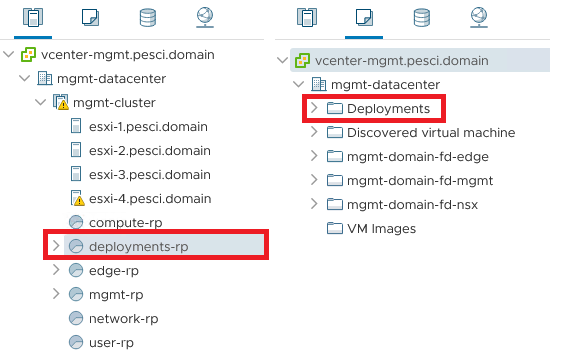
\includegraphics[width=0.6\textwidth]{imaxes/pruebaconcepto/vrealize/rp-vra.png}
        \caption{Resource pool (izquierda) y carpeta (derecha) creadas para alojar las VMs desplegadas desde vRA.}
        \label{fig:rp-folder-vra}
    \end{figure}
    \FloatBarrier
    % Para que las VMs creadas por los usuarios tengan acceso a la red, se crea un nuevo Segment en el router virtual Tier-1 de VMware NSX-T (Figura \ref{fig:two-tier-topology}) donde se alojará una subred dedicada exclusivamente a ser consumida por los usuarios. Al generar el Segment los componentes de VMware NSX-T comunican al router VyOS la nueva ruta mediante el protocolo de enrutamiento BGP, por lo tanto no es necesario aplicar ninguna configuración adicional en los recursos de red físicos.
    La red utilizada para dar acceso a las VMs creadas por los usuarios es el Segment \textit{Mgmt-Region01A-VXLAN} disponible en VMware NSX-T\footnote{Figura \ref{fig:two-tier-topology}}, el cual cuenta con un servidor DHCP\footnote{Como se observa en la figura \ref{fig:topology-segment-mgmt}, el servidor DHCP está gestionado por VMware NSX-T ya que forma parte de sus servicios de red.} y así poder establecer la configuración IP automáticamente de cada nueva VM que se conecte a este Segment. Si fuera necesario, el administrador del SDDC podría generar un Segment diferente en VMware NSX-T por cada proyecto que se cree en vRA, y así separar la red de las VMs de un proyecto del resto de proyectos. Para ello, el administrador crearía un Segment en VMware NSX-T y lo añadiría a vRA. Posteriormente, durante la elaboración de los diseños en vRA se debería hacer referencia al Segment creado específicamente para ese proyecto.
    \begin{figure}[h]
        \centering
        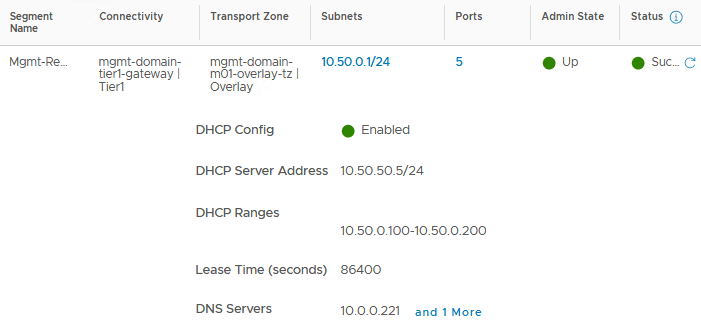
\includegraphics[width=0.7\textwidth]{imaxes/pruebaconcepto/vrealize/segment-MGMT.png}
        \caption{Segment utilizado para el despliegue de VMs con vRA (arriba) y la configuración del servidor DHCP definida en VMware NSX-T (abajo)}
        \label{fig:topology-segment-mgmt}
    \end{figure}
    \FloatBarrier
    % \begin{figure}[h]
    %     \centering
    %     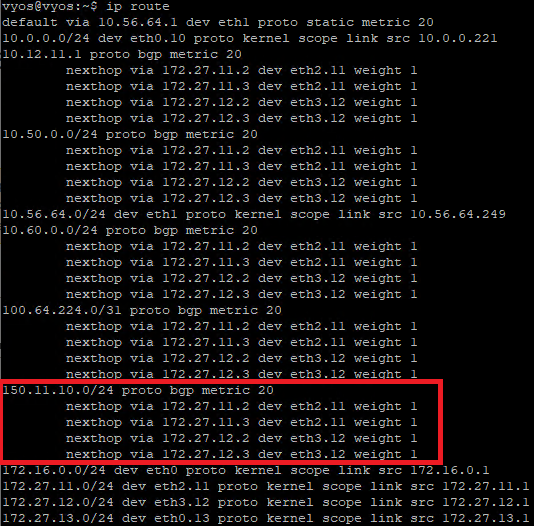
\includegraphics[width=0.4\textwidth]{imaxes/pruebaconcepto/vrealize/router-vyos-bgp.png}
    %     \caption{Nueva ruta configurada en el router VyOS mediante BGP.}
    %     \label{fig:bgp-router-vyos}
    % \end{figure}
    % \FloatBarrier   
    Para que los usuarios tengan plantillas a partir de las cuales generar sus propias VMs, el administrador del SDDC debe crearlas antes. Este proceso consiste en crear una VM, inicializarla con la instalación de un sistema operativo y establecer una configuración base para finalmente generar una plantilla. En el entorno de pruebas se crean dos plantillas de dos sistemas operativos distintos desde VMware vCenter Server, una con Windows Server 2016 (figura \ref{fig:windows-server-installing}) y otra con CentOS 8 (figura \ref{fig:centos-installing}). Una vez instalados ambos sistemas se habilita al menos un método de acceso, SSH en el caso de CentOS y RDP en Windows Server, y se instala el servicio \textbf{cloud-init}\footnote{Ejemplos de uso y su documentación se pueden encontrar en el siguiente enlace: \url{https://cloudinit.readthedocs.io/en/latest/topics/examples.html}.} el cual permitirá a los usuarios finales ejecutar comandos de configuración durante el despliegue de una VM para adaptarla a sus requisitos. En sistemas operativos Windows este servicio se llama \textbf{cloudbase-init}\footnote{Su documentación se puede encontrar en el siguiente enlace:\url{https://cloudbase.it/cloudbase-init/}.}. Una vez se ha completada la configuración se deben ejecutar una serie de comandos, que en el caso de Windows Server son ejecutados directamente por el instalador de cloudbase-init a través del servicio \textbf{sysprep}, para limpiar el sistema y así generar una VM única cada vez que el usuario final utiliza la plantilla. Esto incluye el borrado de paquetes obsoletos y limpieza de logs, claves SSH e identificadores del sistema como direcciones MAC. Una vez se ha completado el proceso se genera una plantilla de cada VM (figura \ref{fig:templates}).
    % Las plantillas empleadas por los usuarios para generar VMs son generadas por el administrador del SDDC. Para crear una plantilla el administrador debe antes crear una VM, instalar en ella el sistema operativo deseado y establecer una configuración inicial. En el entorno de pruebas, dentro del cluster vSphere, se crea una VM con el sistema operativo Ubuntu Server 18.04, para inicializarla se instalan las actualizaciones correspondientes y se configura el servicio \textbf{cloud-init}, el cual permitirá al usuario especificar comandos en el diseño para inicializar automaticamente una VM con los requisitos que desee (instalación de paquetes, creación de usuarios, generación de claves SSH, configuración de red y mucho más\footnote{En el siguiente enlace se pueden encontrar más información sobre cloud-init y ejemplos sobre sus usos: \url{https://cloudinit.readthedocs.io/en/latest/topics/examples.html}}). Una vez configurada se procede a ejecutar un script\footnote{El script se puede encontrar en el anexo .} para limpiar la VM para que cada vez que se utilice la plantilla se genere una VM distinta. Finalmente la VM se convierte a una plantilla que se almacena en VMware vCenter Server. 
    % Siguiendo un procedimiento similar se crea una plantilla a partir de una VM con Windows Server 2016 y otra plantilla con CentOS 8.
    \begin{figure}[h]
        \centering
        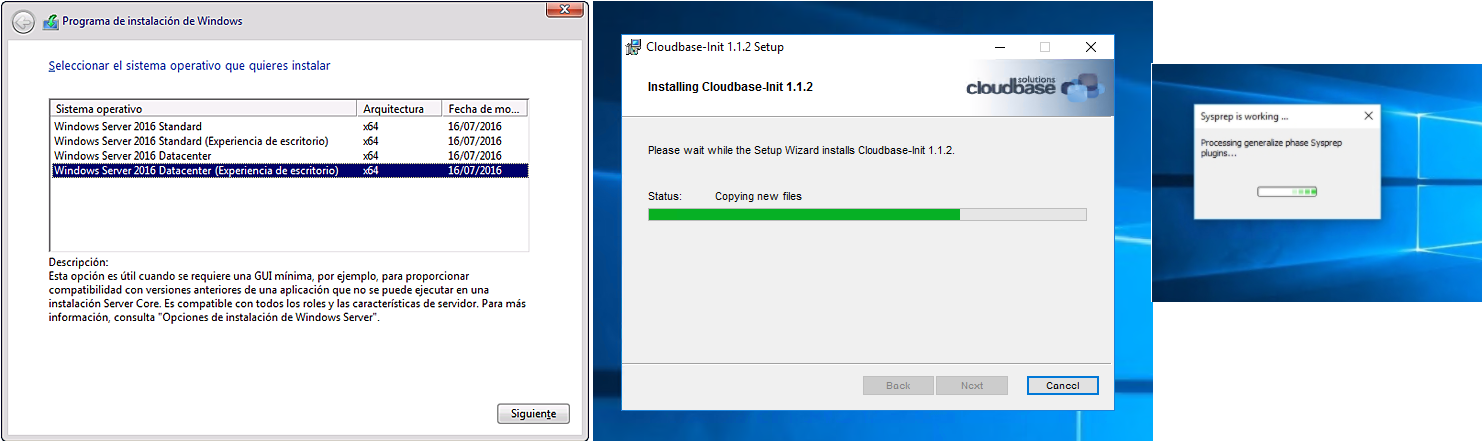
\includegraphics[width=1\textwidth]{imaxes/pruebaconcepto/vrealize/instalador-windows.png}
        \caption{Instalación y preparación de la VM con Windows Server 2016 para la creación de una plantilla}
        \label{fig:windows-server-installing}
    \end{figure}
    \FloatBarrier
    \begin{figure}[h]
        \centering
        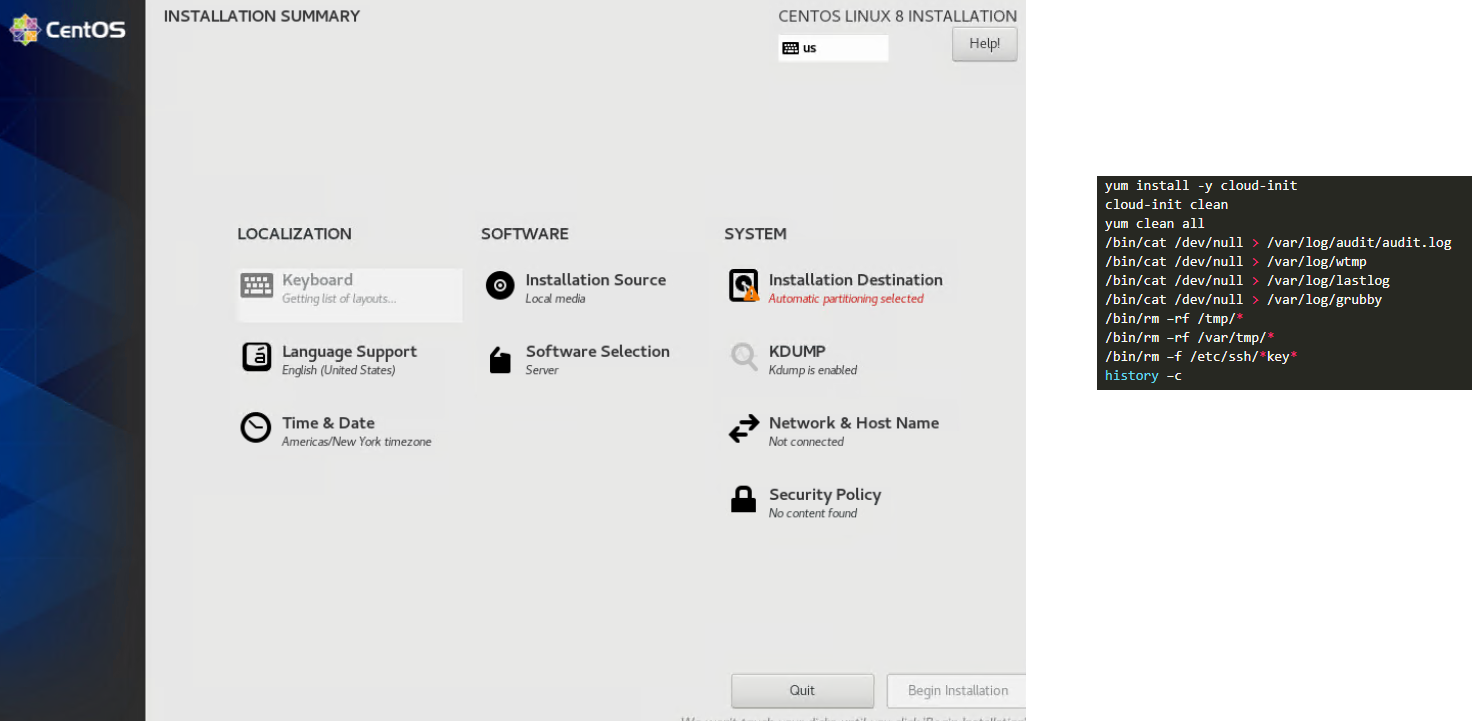
\includegraphics[width=1\textwidth]{imaxes/pruebaconcepto/vrealize/centos-installation.png}
        \caption{Instalación CentOS y comandos ejecutados para la creación de una plantilla.}
        \label{fig:centos-installing}
    \end{figure}
    \FloatBarrier
    \begin{figure}[h]
        \centering
        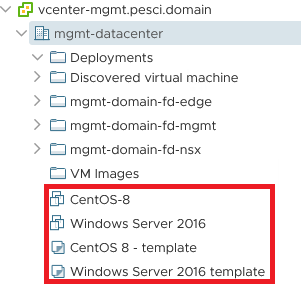
\includegraphics[width=0.4\textwidth]{imaxes/pruebaconcepto/vrealize/plantillas-creadas-vcenter.png}
        \caption{Plantillas de CentOS 8 y Windows Server 2016 creadas a partir de sus respectivas VMs.}
        \label{fig:templates}
    \end{figure}
    \FloatBarrier
    % Se crea otra VM con el sistema operativo Windows Server 2016. En este caso, en lugar de cloud-init se utiliza el servicio \textit{cloudbase-init}\footnote{La documentación de cloudbase-init se puede encontrar aquí: \url{https://cloudbase.it/cloudbase-init/}} que cumple la misma función que el anterior. Una vez completada la instalación y configuración de Windows Server 2016, desde VMware vCenter Server se convierte la VM en una plantilla.
    % \begin{figure}[h]
    %     \centering
    %     \includegraphics[width=0.6\textwidth]{imaxes/pruebaconcepto/vrealize/instalación-cloudbase-windows.png}
    %     \caption{instalación de cloudbase-init en Windows Server 2016.}
    %     \label{fig:cloudbase-init}
    % \end{figure}
    % \FloatBarrier 

    \end{subsubsection}

    \begin{subsubsection}{Configuración de VMware vRealize Automation}
        Para que los recursos de cómputo, red y almacenamiento de la infraestructura sean consumidos por los usuarios, es necesario habilitarlos en la plataforma de vRA. A medida que se integra cada recurso se le asigna uno o más tags para poder identificarlo y que el usuario lo pueda incluir en sus diseños.
        \\ 
        En la siguiente figura se muestran las plantillas creadas anteriormente en VMware vCenter Server. Cada vez que un usuario quiera crear una VM deberá indicar a partir de qué plantilla quiere generarla.
        \begin{figure}[h]
            \centering
            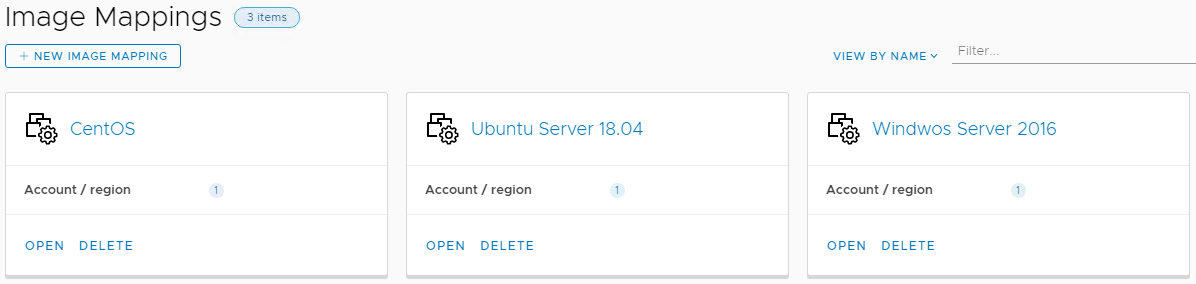
\includegraphics[width=0.7\textwidth]{imaxes/pruebaconcepto/vrealize/image-mappings.png}
            \caption{Plantillas de CentOS 8 y Windows Server 2016 disponibles en vRA.}
            \label{fig:image-mapping}
        \end{figure}
        \FloatBarrier
        Para habilitar el Segment \textit{Mgmt-Region01A-VXLAN}, en vRA se crea un perfil de red y dentro de este se añade la subred deseada. A esta se le asignan los tags \textit{subnet-cidr:10.50.0.0/24}, \textit{function:pro} y \textit{env:pro} como se muestra en la siguiente figura.
        % El Segment configurado en VMware NSX-T se añade como un perfil de red en vRA. Este Segment contiene un servidor DHCP configurado, pero existe la posibilidad de crear un rango de direcciones IP para asignar una IP estática a cada VM que utiliza este perfil. A la subred se le han asignado los tags .
        % , pero en este caso se utiEn este perfil se ha creado un rango de direcciones IP para que vRA asigne una dirección estática a cada VM que lo utilice, y se le han asignado los tags \textit{function: pro} y \textit{env: pro}.
        \begin{figure}[h]
            \centering
            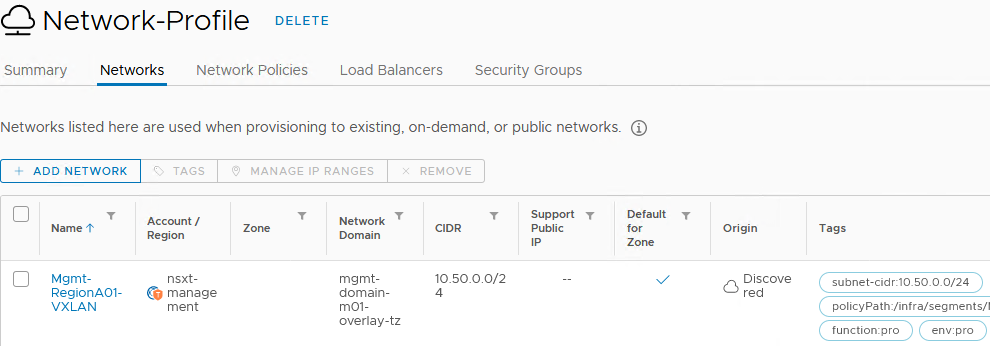
\includegraphics[width=0.8\textwidth]{imaxes/pruebaconcepto/vrealize/net-profile-MGMT.png}
            \caption{Subred habilitada en vRA que se corresponde con el Segment \textit{Mgmt-Region01A-VXLAN} configurado en VMware NSX-T.}
            \label{fig:net-profile}
        \end{figure}
        \FloatBarrier
        Los recursos de cómputo se habilitan configurando una Cloud Zone que se muestra en la figura \ref{fig:cloud-zone}. Esta integra en vRA los recursos del cluster vSphere del entorno y permite establecer la política a seguir para escoger el host donde se debe desplegar cada VM\footnote{La opción DEFAULT escoge un host aleatoriamente.} y la carpeta y resource pool donde se deben colocar. A esta Cloud Zone se le han asignado los tags \textit{cloud: private} y \textit{region: management}, y al resource pool el tag \textit{resource:rpprivate}.
       \begin{figure}[h]
            \centering
            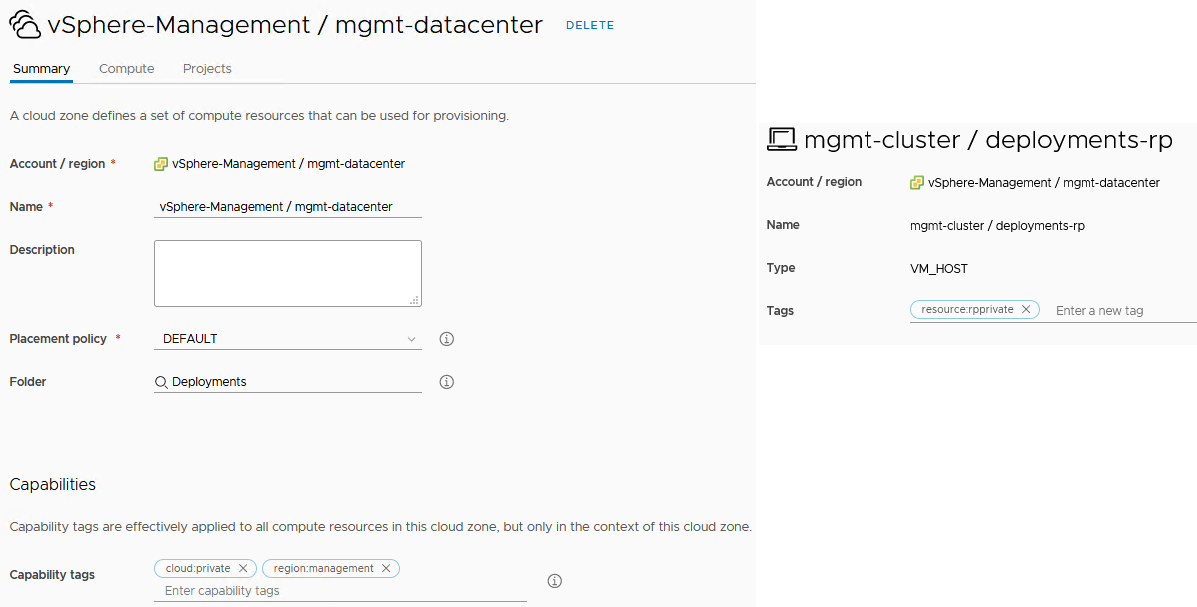
\includegraphics[width=0.8\textwidth]{imaxes/pruebaconcepto/vrealize/cloud-zone.png}
            \caption{Cloud Zone (izquierda) y resource pool (derecha) configurados para utilizar los recursos de cómputo y colocar las VMs desplegadas.}
            \label{fig:cloud-zone}
        \end{figure}
        \FloatBarrier
        Igual que con los recursos de red, para habilitar los recursos de almacenamiento se debe crear un perfil de almacenamiento como se muestra en la figura \ref{fig:storage-policy}. Este perfil integra al datastore vSAN utilizado por el cluster vSphere del entorno y se establece como el perfil por defecto para aprovisionar recursos de almacenamiento desde vRA. Al perfil se le asignan los tags \textit{cloud: private} y \textit{function: pro}.
        % Para el almacenamiento, se crea un perfil que se muestra en la siguiente imagen. Este perfil tiene como recurso de almacenamiento el datastore configurado para el Management Domain, y se establece como el perfil por defecto para el aprovisionamiento de recursos de almacenamiento. Se la han asignado los tags \textit{cloud: private} y \textit{function: pro}. 
        \begin{figure}[h]
            \centering
            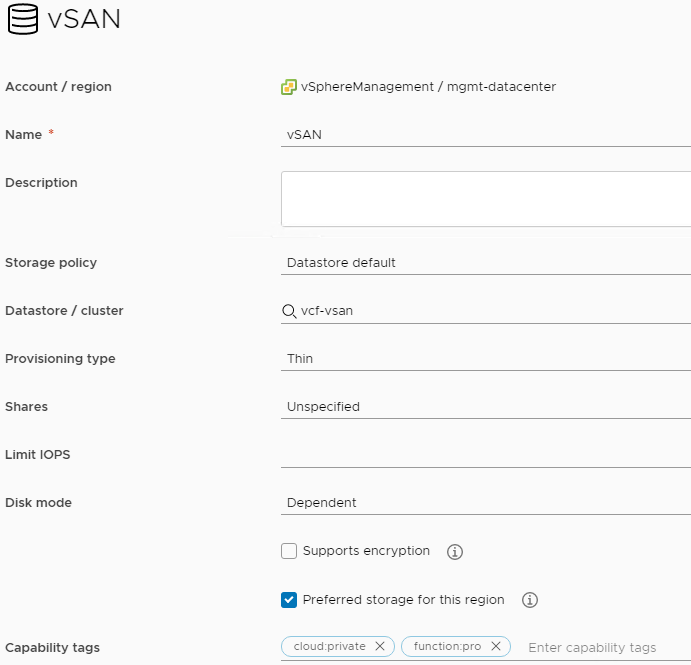
\includegraphics[width=0.6\textwidth]{imaxes/pruebaconcepto/vrealize/datastore-policy.png}
            \caption{Perfil de almacenamiento configurado donde se indica el datastore utilizado para aprovisionar recursos de almacenamiento.}
            \label{fig:storage-policy}
        \end{figure}
        \FloatBarrier
        Además, el administrador del SDDC define varios perfiles de tamaños para que los usuarios determinen el tamaño de sus VMs. En estos perfiles se define una cantidad de CPU y memoria RAM con el fin de estandarizar la cantidad de recursos que un usuario puede asignar a una VM. En el entorno de pruebas, estos tamaños van desde \textit{x-small} con 1 CPU y 512 MB de memoria RAM, hasta \textit{large} con 8 CPUs y 16 GB de memoria RAM, mostrados en la siguiente figura.
        \begin{figure}[h]
            \centering
            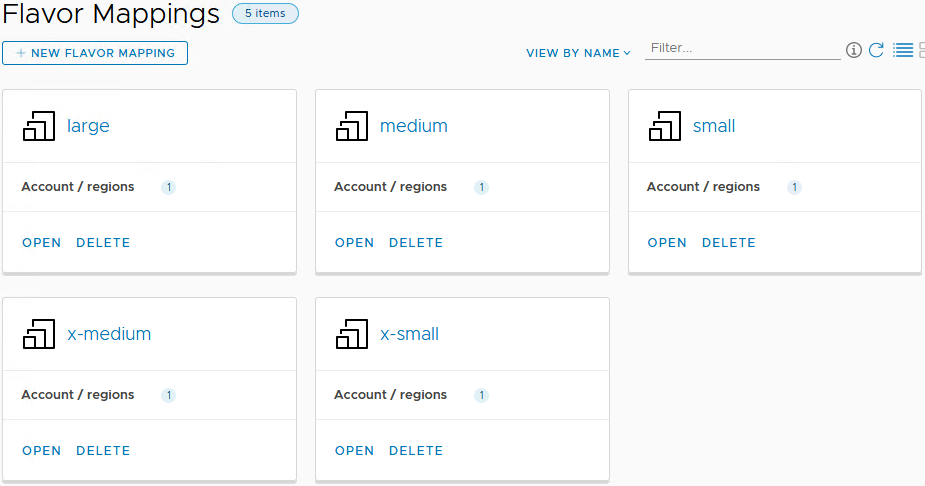
\includegraphics[width=0.6\textwidth]{imaxes/pruebaconcepto/vrealize/flavor-mapping.png}
            \caption{Perfiles donde se preestablecen la cantidad de recursos que puede tomar una VM.}
            \label{fig:falvor-mapping}
        \end{figure}
        \FloatBarrier
        Con el objetivo de establecer una valoración de los recursos que utilizan los usuarios, se hace uso de las tarjetas de cobro. Se define una única tarjeta que se aplicará a todos los proyectos que se creen en la plataforma, y a medida que se vayan desplegando VMs se generará un cálculo total en base al precio asignado a cada recurso, a la cantidad de recursos utilizados y al tiempo que el despliegue se mantiene activo. Tanto el administrador del SDDC como el usuario tendrán acceso a estadísticas sobre el gasto que se realiza y de la cantidad total de recursos utilizados. En la figura \ref{fig:pricing-card} se muestra la valoración establecida para el consumo de recursos, que es de 1 €/hora por cada CPU cuando la VM está encendida, 2 €/hora por cada GB de memoria RAM cuando la VM está encendida y 0,5 €/hora por GB de almacenamiento mientras el despliegue esté activo. 
        \begin{figure}[h]
            \centering
            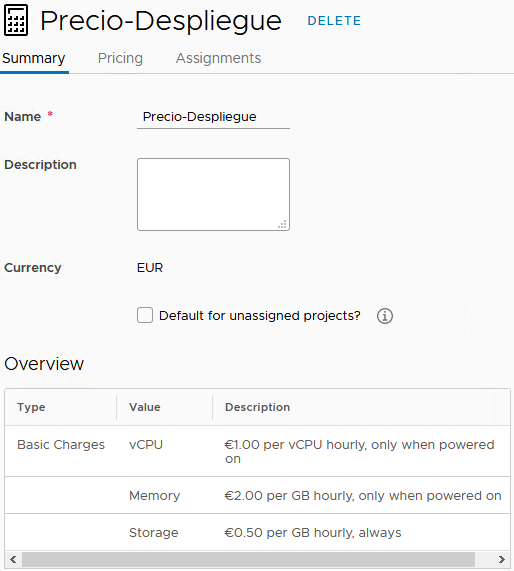
\includegraphics[width=0.6\textwidth]{imaxes/pruebaconcepto/vrealize/pricing-card.png}
            \caption{Tarjeta de cobro para valorar los recursos consumidos por los usuarios.}
            \label{fig:pricing-card}
        \end{figure}
        \FloatBarrier

    \end{subsubsection}

    \begin{subsubsection}{Uso del servicio Cloud}
        La plataforma de vRA ya está lista para ser utilizada por los usuarios. Los usuarios del CITIC que la utilizarán se organizan en proyectos, donde existe al menos un coordinador o administrador de proyecto. Cuando un grupo de usuarios quiere utilizar el servicio Cloud primero debe comunicarlo al administrador del SDDC, el cual crea el proyecto correspondiente y habilita el acceso a cada usuario con sus correspondientes permisos.

        % Como ya se ha visto en la sección \nameref{subsubsec:WSA}, 
        En el entorno de pruebas el administrador ha configurado dos proyectos con sus respectivos usuarios, uno llamado Web-DB con el objetivo de que los usuarios pertenecientes puedan construir un sitio web bajo demanda, y otro llamado Server-Desktop donde sus integrantes puedan desplegar dos VMs para realizar cierto trabajo de investigación (figura \ref{fig:projects-vra}). El proyecto Web-DB lo forman el usuario \textit{User One}, \textit{User Two} y \textit{Manager One}, el cual es el coordinador del grupo, y el proyecto Server-Desktop está formado por \textit{User Two}, \textit{User Three} y \textit{Manager Two}, el cual será el coordinador de este segundo grupo. Entonces, a los usuarios \textit{Manager One} y \textit{Manager Two} se les asigna el rol Administrador de Proyecto, y al resto de usuarios el rol Miembro de Proyecto, los primeros podrán controlar los diseños disponibles en el catálogo del proyecto, qué usuarios tienen acceso y los despliegues que estos realicen, mientras que los miembros del proyecto podrán desplegar los diseños habilitados (figura \ref{fig:project-users}).
        \begin{figure}[h]
            \centering
            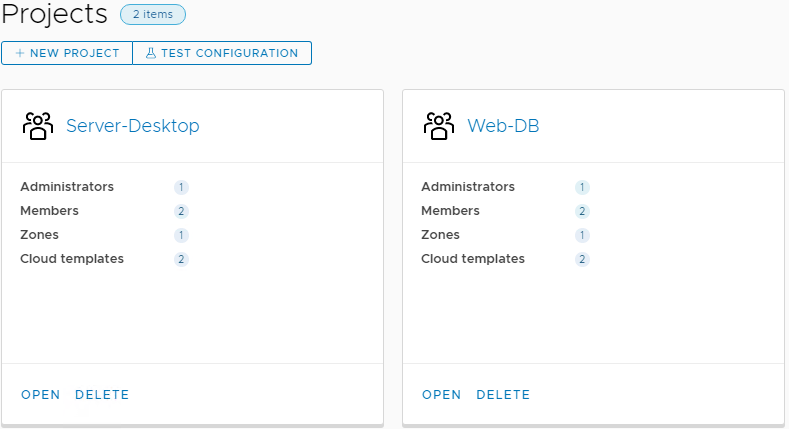
\includegraphics[width=0.6\textwidth]{imaxes/pruebaconcepto/vrealize/projects-vRA.png}
            \caption{Proyectos creados por el administrador del SDDC para dar acceso a los usuarios a vRA.}
            \label{fig:projects-vra}
        \end{figure}
        \FloatBarrier
        \begin{figure}[h]
            \centering
            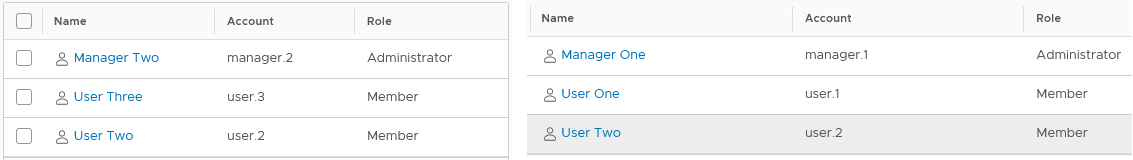
\includegraphics[width=0.6\textwidth]{imaxes/pruebaconcepto/vrealize/users-DB.png}
            \caption{Usuarios del proyecto Server-Desktop (izquierda) y usuarios del proyecto Web-DB (derecha).}
            \label{fig:project-users}
        \end{figure}
        \FloatBarrier
        Durante la creación de los proyectos el administrador establece la cantidad máxima de CPU, memoria RAM y almacenamiento que pueden consumir en total los usuarios del proyecto. Como se trata de un entorno de pruebas en el proyecto Server-Desktop se establece un límite de 2 VMs, 10 GB de memoria RAM y 6 CPUs, y en el proyecto Web-DB un límite de 3 VMs, 10 GB de memoria RAM y 6 CPUs, de esta forma los usuarios del proyecto no podrán superar ninguno de los límites establecidos. Para obtener una valoración del consumo se asigna a cada proyecto la tarjeta de cobro creada anteriormente.
        % Cuando el administrador crea un proyecto establece la cantidad máxima de CPU, memoria RAM y almacenamiento que puede consumir en total. También se pueden establecer mediante el uso de tags, los recursos que los despliegues del proyecto deben utilizar por defecto.
        \\
        Una vez configurados ambos proyectos los administradores de cada uno pueden acceder y empezar a crear los diseños de los recursos que requieran sus usuarios a través del componente Cloud Assembly. El administrador del proyecto Server-Desktop, \textit{Manager Two}, crea el diseño con el nombre WD-Server que se muestra en la siguiente figura\footnote{En el anexo \ref{appendix:wd-server-blueprint} se encuentra el contenido del archivo .yaml donde se establece la configuración del diseño.}.
        \begin{figure}[h]
            \centering
            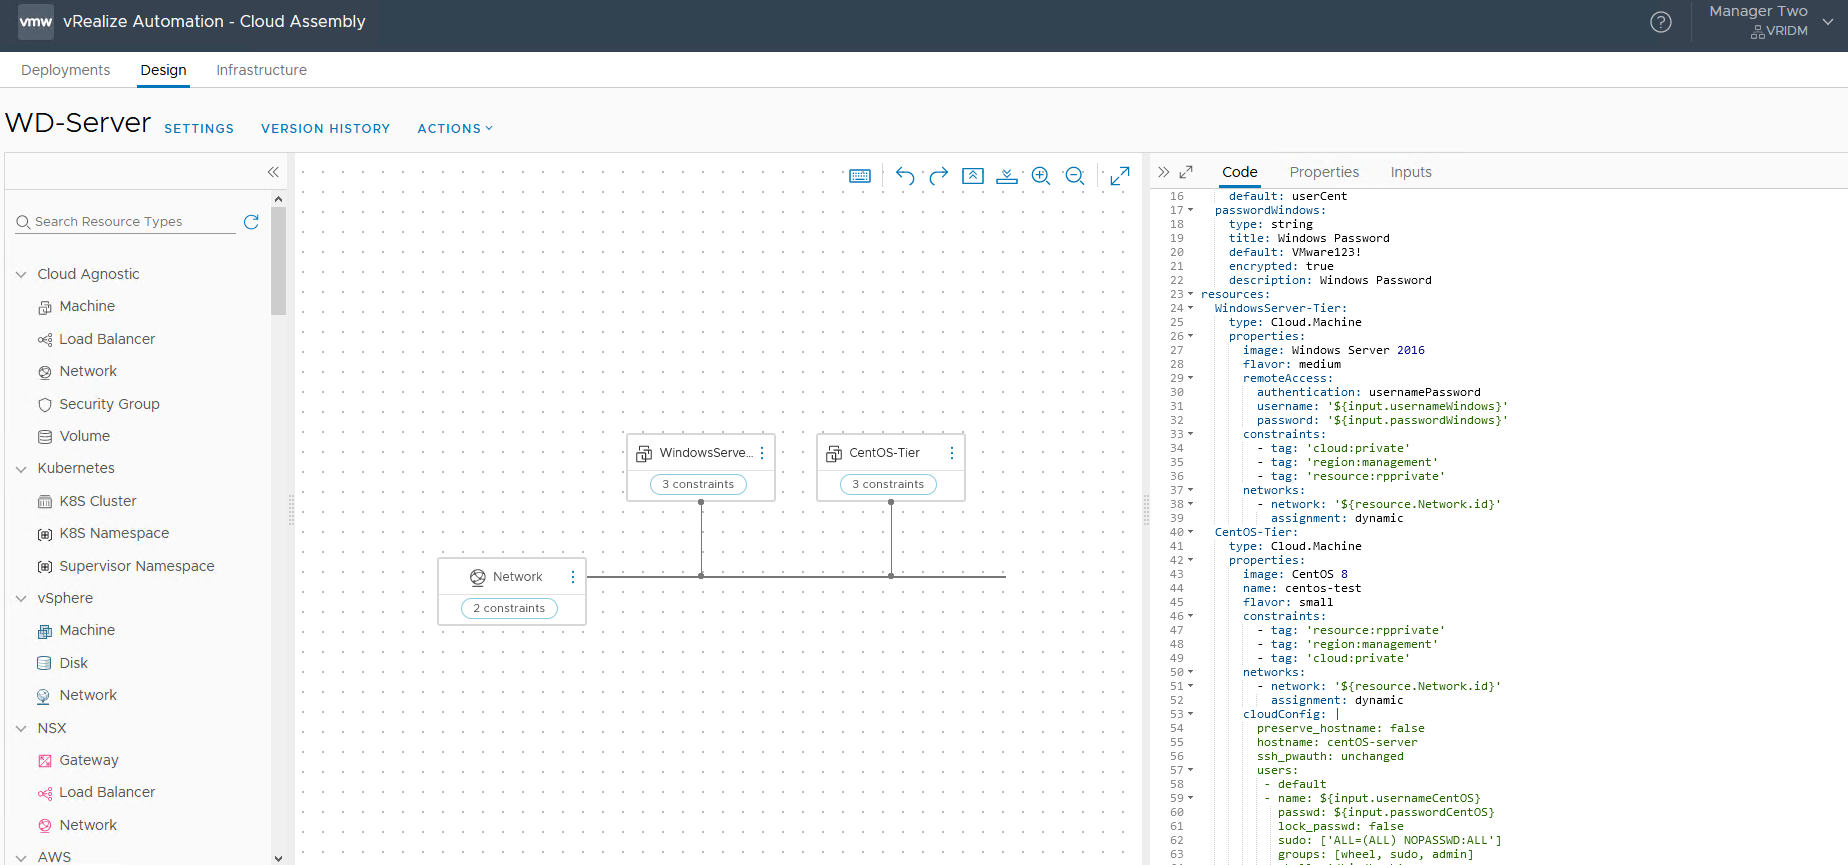
\includegraphics[width=0.8\textwidth]{imaxes/pruebaconcepto/vrealize/windows-centos-blueprint.png}
            \caption{Diseño WD-Server para el proyecto Server-Desktop.}
            \label{fig:server-desktop-blueprint}
        \end{figure}
        \FloatBarrier
        En el archivo .yaml del diseño WD-Server se define una VM con el sistema operativo Windows Server 2016 y otra con CentOS 8, y una red a la que ambas se conectan. Se establecen además unas credenciales para cada VM, cuyos datos son introducidos por el usuario cuando se despliega el diseño y así poder iniciar sesión en ellas mediante SSH, o RDP en el caso de Windows. Los tags que se utilizan en la definición de las VMs son \textit{cloud:private}, \textit{region:management} y \textit{resource:rpprivate}, y el tag \textit{subnet-cidr:10.50.0.0/24} en la definición de la red, por lo tanto ambas VMs utilizarán los recursos del cluster vSphere, el Segment definido en VMware NSX-T y el datastore vSAN del entorno. En cuanto a la configuración de las interfaces de red, se establece que se configuren de forma dinámica con el servidor DHCP disponible en el Segment. Una vez completado el diseño, \textit{Manager Two} publica el diseño en el catálogo del proyecto para que los usuarios puedan acceder a él. Durante la publicación se especifica la versión del diseño ya que este puede ser actualizado, como se muestra en la siguiente figura.
        \begin{figure}[h]
            \centering
            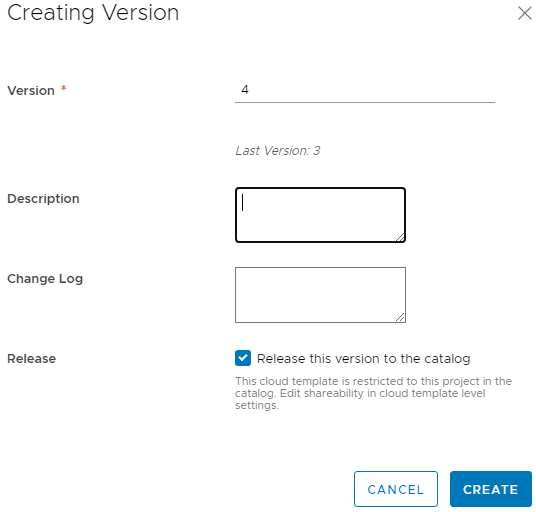
\includegraphics[width=0.6\textwidth]{imaxes/pruebaconcepto/vrealize/create-version-blueprint.png}
            \caption{Publicación en el catálogo de una nueva versión del diseño.}
            \label{fig:publication-version}
        \end{figure}
        \FloatBarrier
        De la misma forma que para el proyecto Server-Desktop, el administrador del proyecto Web-WD, \textit{Manager One}, crea el diseño de los recursos necesarios para que los usuarios del proyecto puedan generar un sitio web basado en Wordpress automatizando la configuración del entorno, con la idea de que una vez desplegados los recursos el usuario pueda trabajar inmediatamente y exclusivamente en su sitio web. En la siguiente figura se muestra el diseño creado para el proyecto Web-WD\footnote{En el anexo \ref{appendix:worpress-mysql-blueprint} se encuentra el contenido del archivo .yaml donde se establece la configuración del diseño.}.
        \begin{figure}[h]
            \centering
            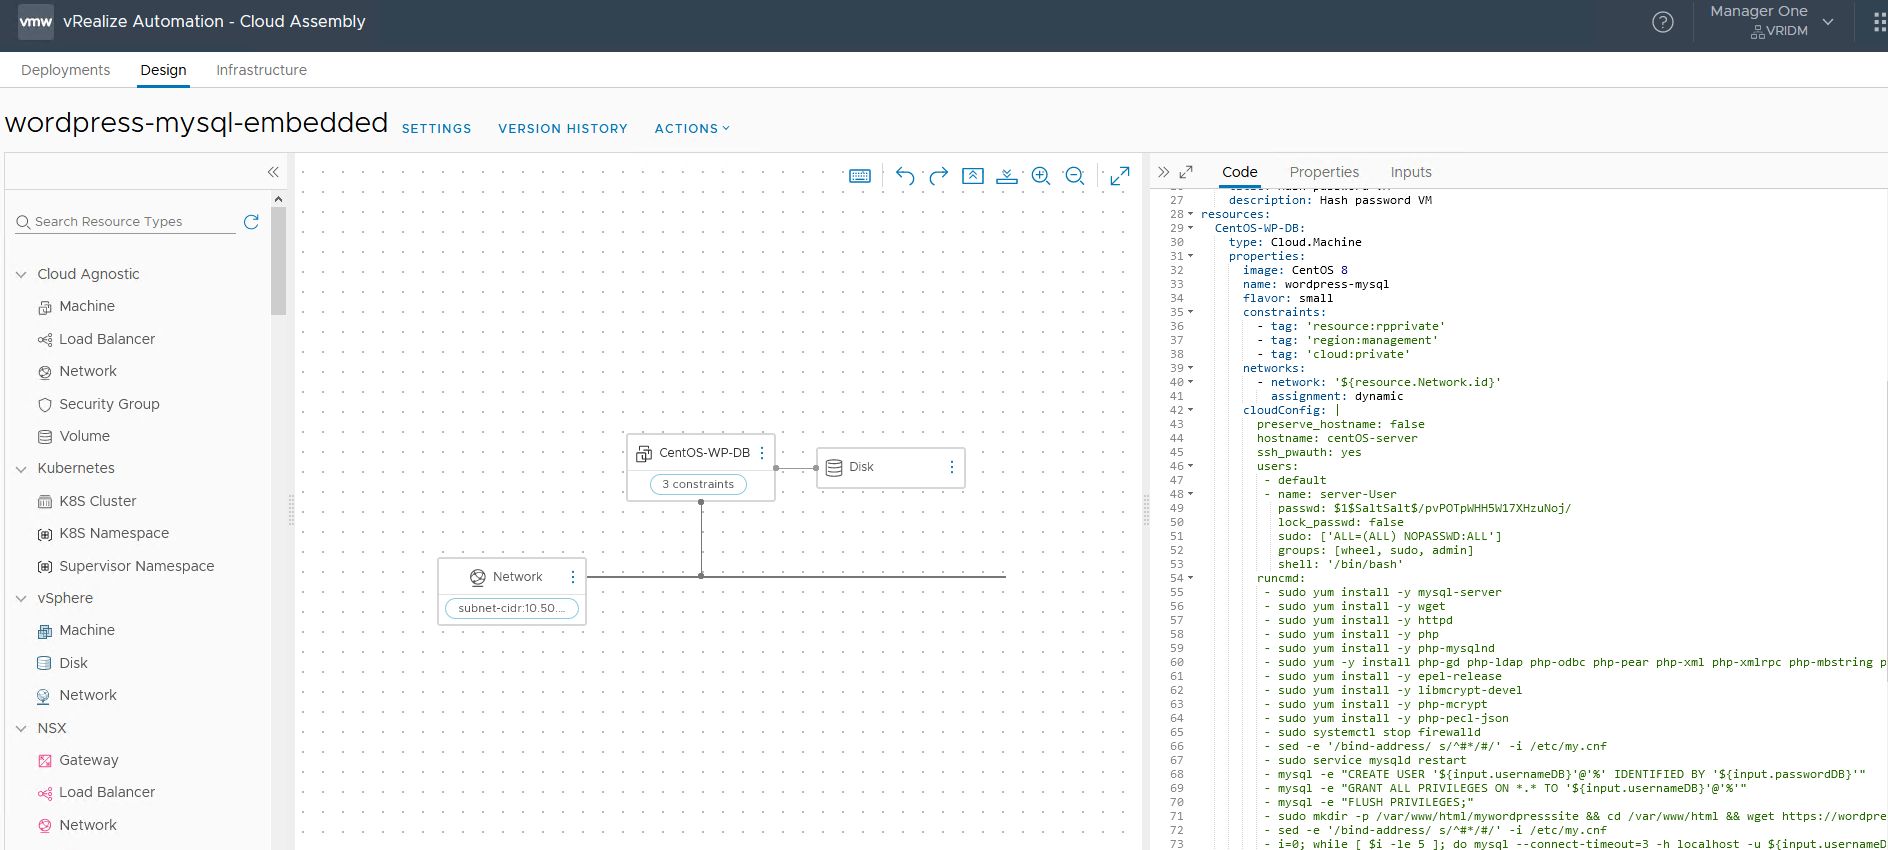
\includegraphics[width=0.8\textwidth]{imaxes/pruebaconcepto/vrealize/wordpress-mysql-blueprint.png}
            \caption{Diseño Wordpress-MySQL-Embedded para el proyecto Web-WD.}
            \label{fig:web-WD-blueprint}
        \end{figure}
        \FloatBarrier
        En el archivo .yaml del diseño Wordpress-MySQL-Embedded se define una VM con el sistema operativo CentOS 8, una red a la cual se conecta y un disco de almacenamiento conectado a la VM. En la sección \textbf{cloudConfig} del diseño se definen una serie de comandos que se ejecutan durante la inicialización de la VM cuando se despliega. Estos comandos son ejecutados por el servicio \textbf{cloud-init} y con ellos primero se instalan los paquetes necesarios para ejecutar MySQL y el framework Wordpress en un servidor Apache, luego se crea una base de datos y se configura Wordpress. De esta forma una vez se complete un despliegue el sitio web estará listo para ser usado. Además también se incluyen en esa sección del diseño los atributos que permiten a cloud-init crear las credenciales para acceder a la VM mediante SSH. Este diseño utiliza los mismos tags que el proyecto Server-Desktop por lo tanto utilizará los mismos recursos de cómputo, red y almacenamiento. Finalmente, \textit{Manager One} publica el diseño en el catálogo.        
        % Durante el despliegue del diseño, en la VM se instala y configura el gestor de base de datos MySQL y el framework web Wordpress. Para ello, se hace uso de la propiedad \textbf{cloudConfig} la cual invoca al servicio \textbf{cloud-init} para la ejecución de los comandos definidos en el diseño, que en este caso se utilizan para descargar los paquetes de MySQL, Wordpress y sus dependencias, y posteriormente crear una base datos, configurar Wordpress para conectarse a ella y habilitar un servidor Apache para acceder al sitio web. Además, también incluye la definición de un usuario para inciar sesión en la VM mediante SSH y de las credenciales usadas para conectarse a la base de datos. Los tags utilizados son los mismos que en el proyecto anterior por lo tanto este diseño se desplegará en la misma ubicación. Finalmente, \textit{Manager One} publica el diseño en el catálogo.        
        \\
        Una vez completada la fase de diseño y publicación, los usuarios ya pueden acceder al servicio Cloud y comenzar a utilizar los recursos en base a los diseños disponibles. A continuación se muestra cómo los usuarios de cada proyecto acceden al servicio Cloud y utilizan los recursos. 
        El usuario \textit{User Three} perteneciente al proyecto Server-Desktop accede a la plataforma utilizando sus credenciales\footnote{En el caso del entorno real utilizaría sus credenciales de la UDC.}, una vez inicia sesión accede al componente Service Broker de vRA donde se le muestra el catálogo de diseños disponibles en el proyecto al que pertenece (figura \ref{fig:login-user-3-catalog}). Cuando inicia el despliegue del diseño WD-Server, se muestra un formulario donde introduce los datos de las credenciales de cada VM\footnote{Para la VM con CentOS es necesario indicar el hash de la contraseña ya que el SO lo interpreta de esta forma, generado en este caso con el comando \textit{openssl passwd -1 -salt SaltSalt VMware123!} desde el powershell de Windows siendo "VMware123!" la contraseña en texto plano.} que se va a crear y el nombre del despliegue (figura \ref{fig:login-user-3-form-deployment}). A continuación comienza el proceso de despliegue. En este punto vRA se encarga de crear, configurar y reservar los recursos descritos en el diseño sin que el usuario tenga que realizar ninguna operación adicional (figura \ref{fig:deployment-process-user-3}).
        \begin{figure}[h]
            \centering
            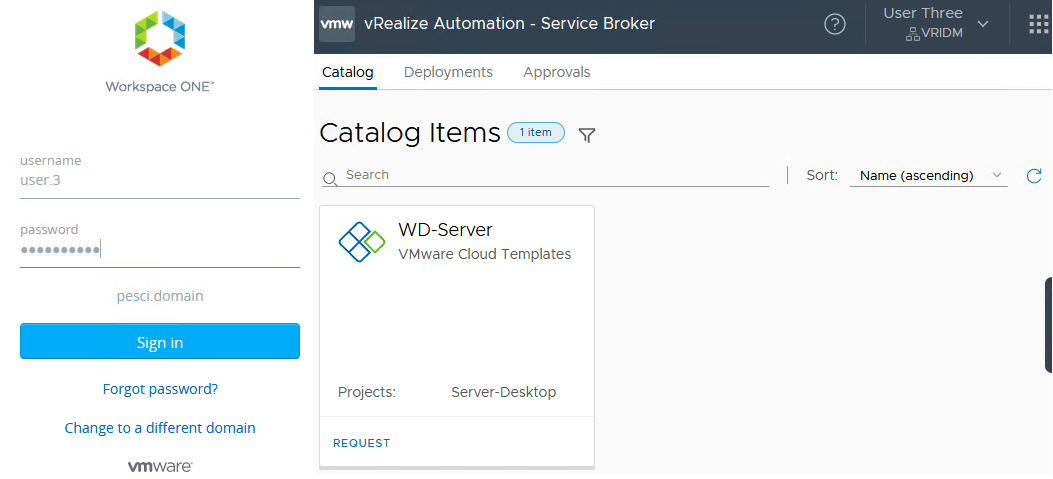
\includegraphics[width=0.7\textwidth]{imaxes/pruebaconcepto/vrealize/login-user-3-credentials.png}
            \caption{Inicio de sesión del usuario \textit{User Three} (izquierda) y catálogo de diseños disponibles en el proyecto Server-Desktop (derecha).}
            \label{fig:login-user-3-catalog}
        \end{figure}
        \FloatBarrier
        \begin{figure}[h]
            \centering
            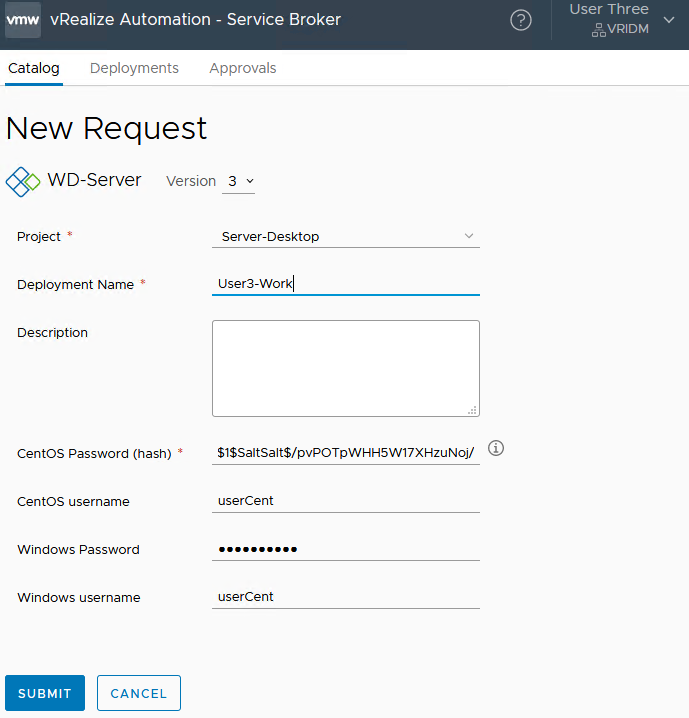
\includegraphics[width=0.6\textwidth]{imaxes/pruebaconcepto/vrealize/deployment-user-3-Windows.png}
            \caption{Formulario para configurar el nuevo despliegue iniciado por el usuario \textit{User Three}.}
            \label{fig:login-user-3-form-deployment}
        \end{figure}
        \FloatBarrier
        \begin{figure}[h]
            \centering
            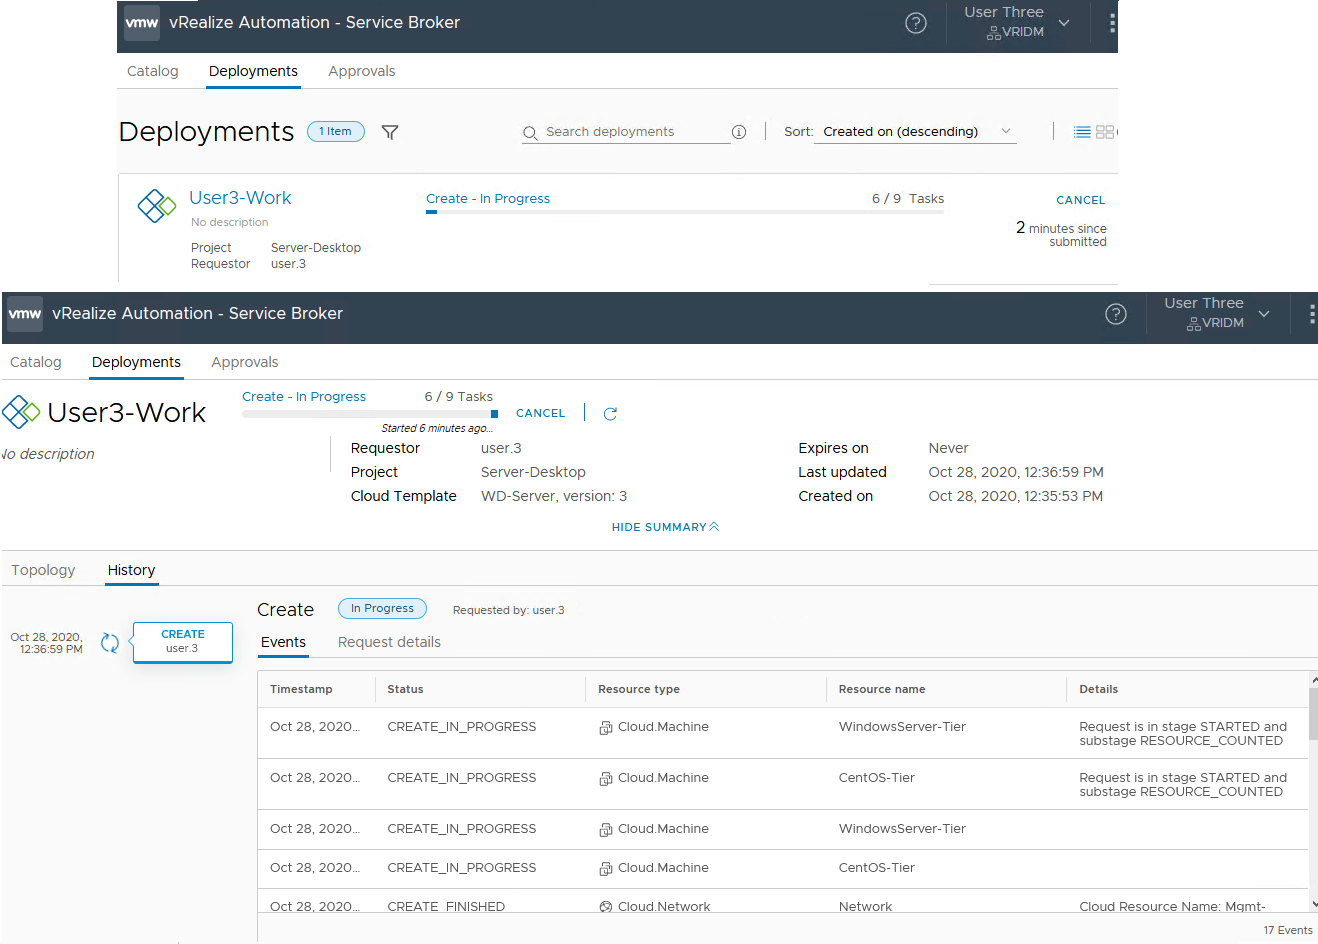
\includegraphics[width=0.8\textwidth]{imaxes/pruebaconcepto/vrealize/deployment-start-user-3-Windows.png}
            \caption{Tarjeta del despliegue iniciado por el usuario \textit{User Three} (arriba) y la monitorización de todas las tareas llevadas a cabo por vRA durante el despliegue (abajo).}
            \label{fig:deployment-process-user-3}
        \end{figure}
        \FloatBarrier
        Cuando la creación y configuración de los recursos se ha completado estos ya están listos para su uso. En el panel de control del despliegue se muestra información como direcciones IP de las VMs, discos de almacenamiento disponibles en cada VM, la configuración aplicada a las VMs durante el despliegue o las credenciales indicadas por el usuario para acceder a las VMs (figura \ref{fig:user3-panel-control}). Además, desde este punto es donde el usuario puede gestionar los recursos pudiendo encenderlos o apagarlos, añadir discos de almacenamiento, modificar el tamaño de la VM, crear copias de seguridad y añadir tags para cambiar la ubicación de los recursos (figura \ref{fig:user3-actions}). Para acceder a las VMs creadas, \textit{User Three} simplemente tiene que comprobar las direcciones IP que se han asignado y conectarse a la VMs mediante SSH o a través de un cliente de escritorio remoto en el caso de Windows Server 2016 (figura \ref{fig:vm-cent-win-connection}).
        \begin{figure}[h]
            \centering
            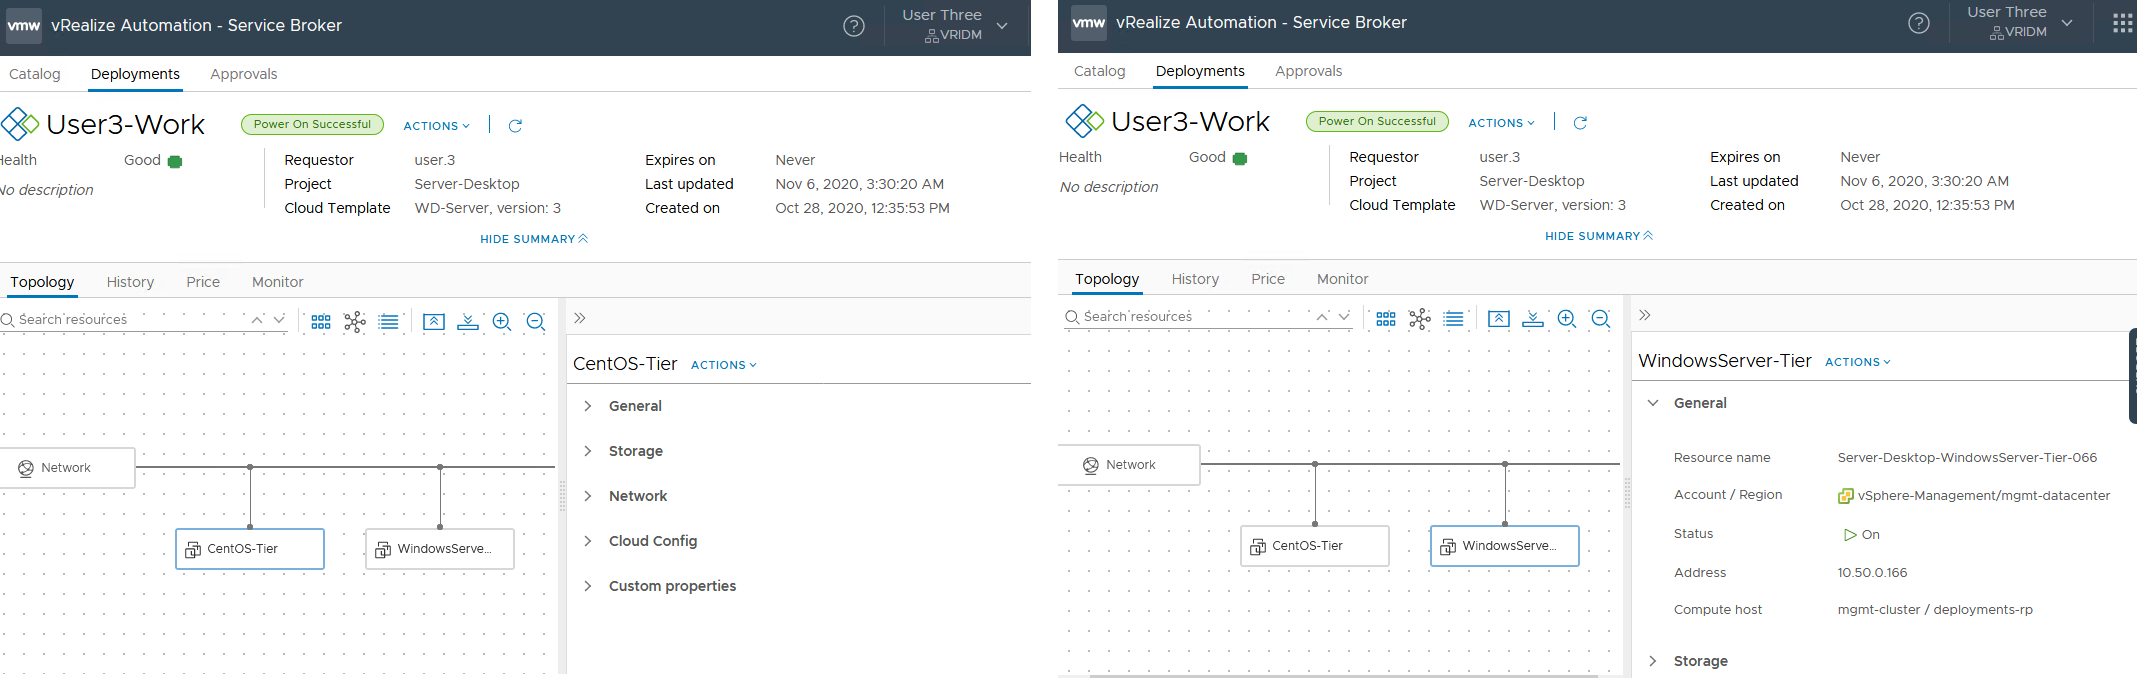
\includegraphics[width=0.8\textwidth]{imaxes/pruebaconcepto/vrealize/user3-info-centos.png}
            \caption{Panel de control de la VM CentOS creada por \textit{User Three} (izquierda) y panel de control de la VM Windows creada por \textit{User Three} (derecha).}
            \label{fig:user3-panel-control}
        \end{figure}
        \FloatBarrier
        \begin{figure}[h]
            \centering
            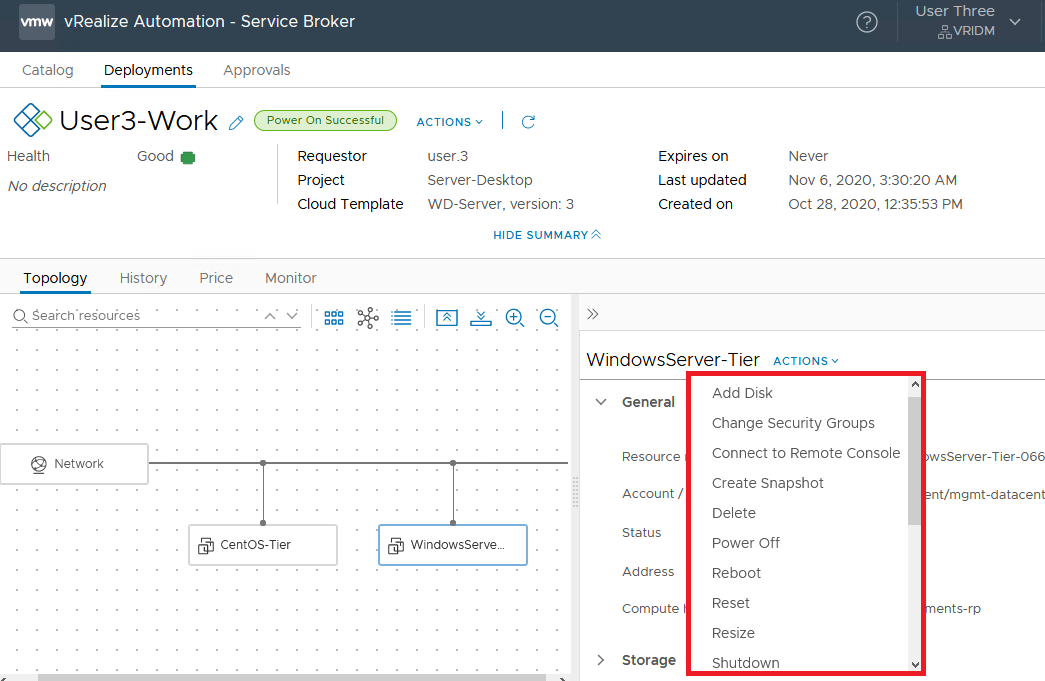
\includegraphics[width=0.7\textwidth]{imaxes/pruebaconcepto/vrealize/user3-vm-actions.png}
            \caption{Acciones que \textit{User Three} puede ejecutar sobre las VMs creadas.}
            \label{fig:user3-actions}
        \end{figure}
        \FloatBarrier
        \begin{figure}[h]
            \centering
            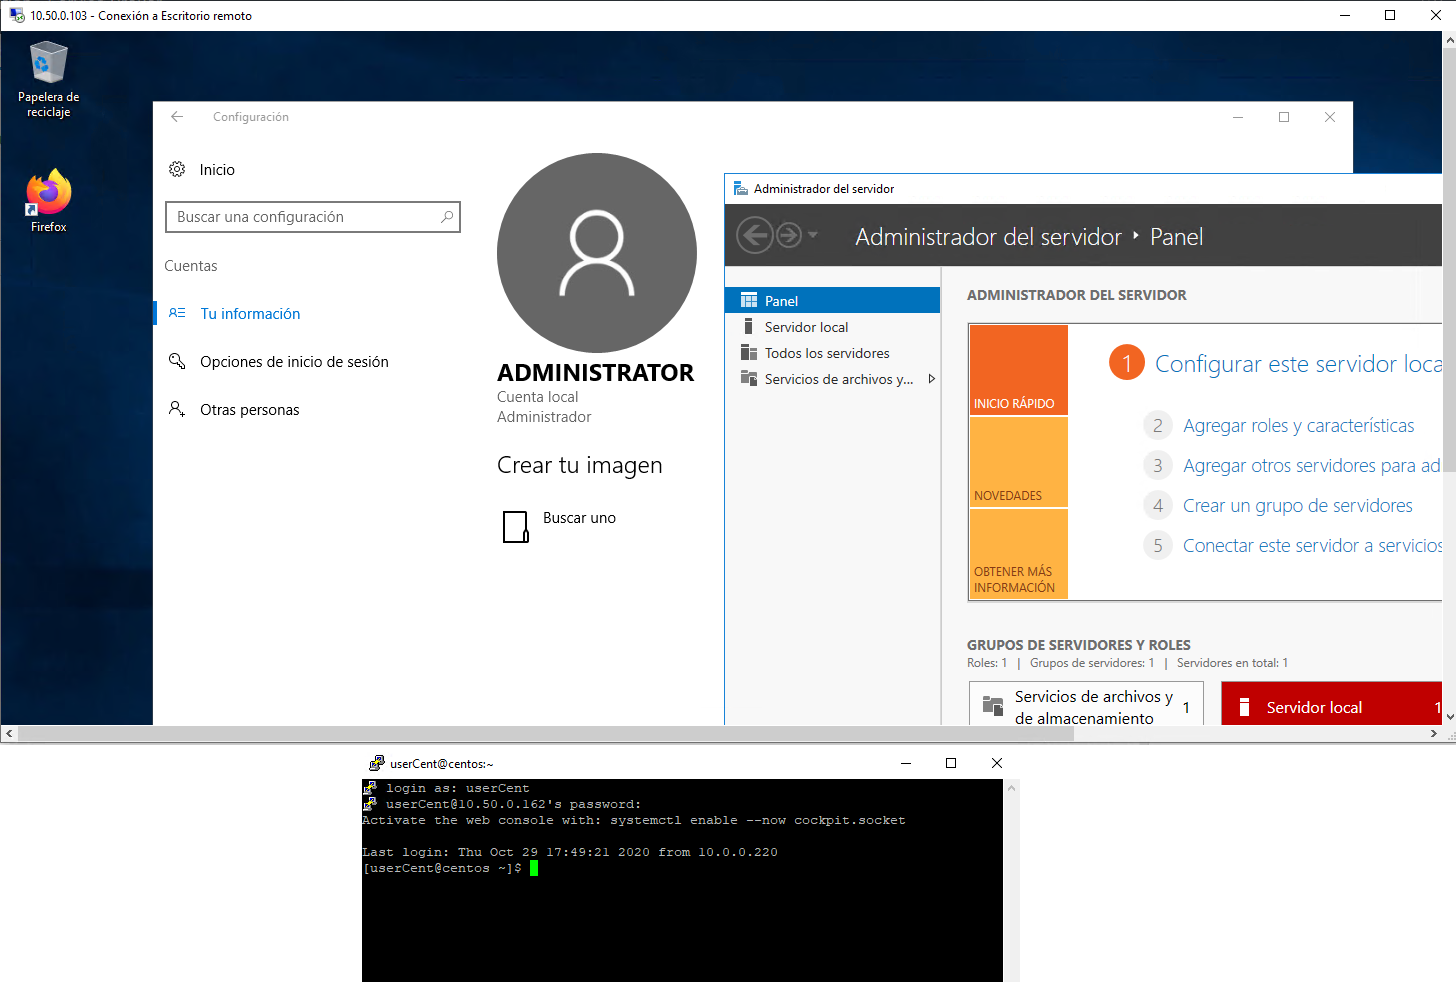
\includegraphics[width=0.7\textwidth]{imaxes/pruebaconcepto/vrealize/Windows-RDP.png}
            \caption{Conexión de \textit{User Three} mediante RDP a la VM con Windows Server 2016 (arriba) y mediante SSH a la VM con CentOS (abajo).}
            \label{fig:vm-cent-win-connection}
        \end{figure}
        \FloatBarrier
        En el proyecto Web-WD, el usuario \textit{User Two} accede a la plataforma de vRA y en el catálogo tiene disponibles dos diseños, WD-Server y Wordpress-MySQL-Embedded, ya que es miembro de los dos proyectos Server-Desktop y Web-WD (figura \ref{fig:catalog-user-2}). El objetivo de este usuario es montar un sitio web por lo tanto inicia el despliegue del diseño Wordpress-MySQL-Embedded. En el formulario de configuración \textit{User Two} introduce las credenciales que se deben configurar en la VM para acceder a ella y para configurar a la base de datos  (figura \ref{fig:catalog-user-2}), luego inicia el despliegue del diseño (figura \ref{fig:deployment-user-2}). Una vez generada la VM con CentOS el servicio cloud-init se inicia y ejecuta los comandos descritos en el diseño (figura \ref{fig:cloud-init-user-2}). Cuando este proceso se ha completado el usuario ya puede acceder al panel de control del despliegue (figura \ref{fig:control-panel-user2}), comprobar la dirección IP de la VM, acceder a Wordpress a través del navegador, realizar la configuración inicial de su sitio web y comenzar a editar artículos (figura \ref{fig:wordpress-user-2}).
        \begin{figure}[h]
            \centering
            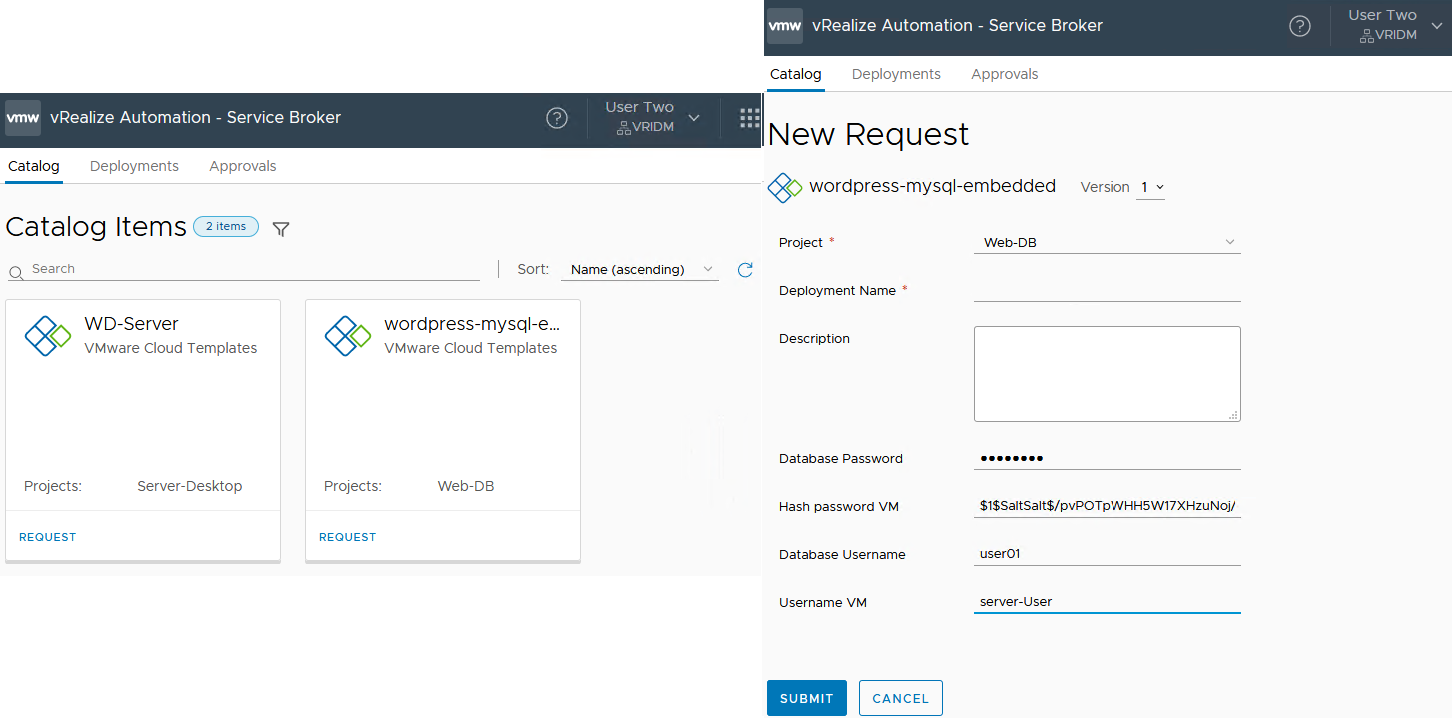
\includegraphics[width=0.7\textwidth]{imaxes/pruebaconcepto/vrealize/user-two-catalog.png}
            \caption{Diseños disponibles para \textit{User Two} (izquierda). Formulario de configuración de un nuevo despliegue del diseño Wordpress-MySQL-Embedded (derecha).}
            \label{fig:catalog-user-2}
        \end{figure}
        \FloatBarrier
        \begin{figure}[h]
            \centering
            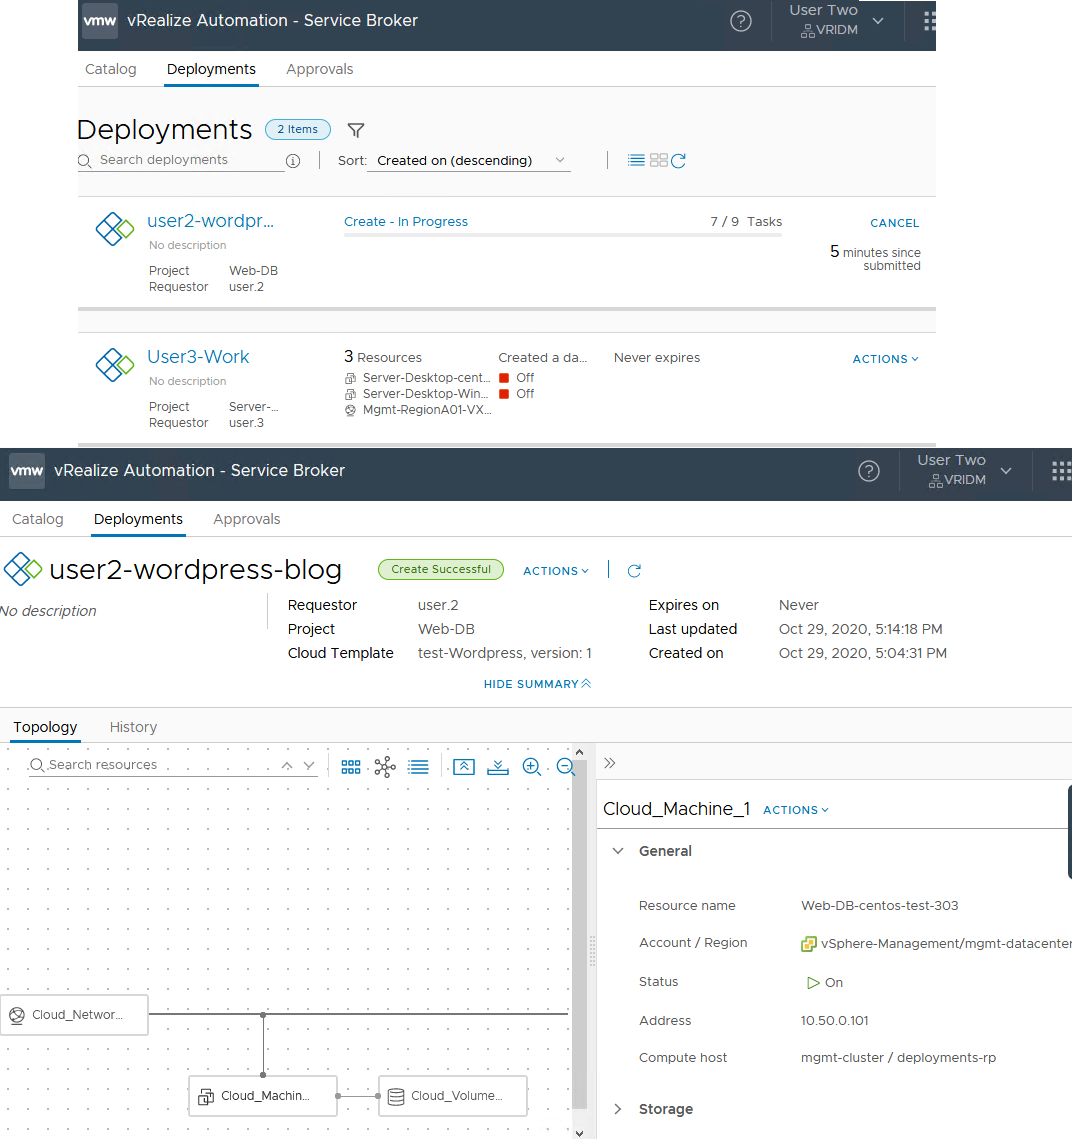
\includegraphics[width=0.7\textwidth]{imaxes/pruebaconcepto/vrealize/user-2-card-deploy.png}
            \caption{Despliegues user2-wordpress-blog iniciado por \textit{User Two}.}
            \label{fig:deployment-user-2}
        \end{figure}
        \FloatBarrier
        \begin{figure}[h]
            \centering
            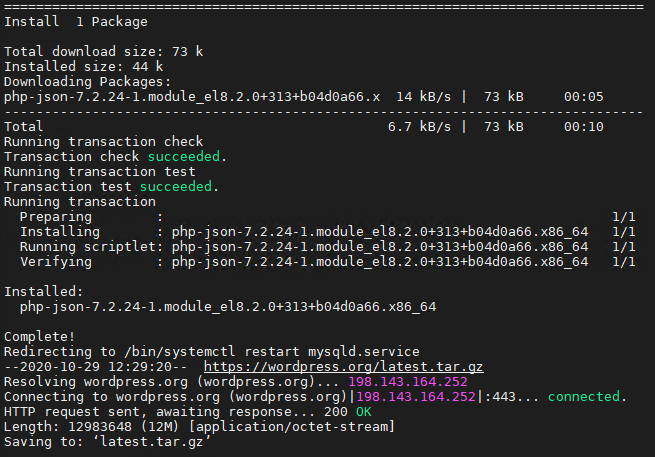
\includegraphics[width=0.6\textwidth]{imaxes/pruebaconcepto/vrealize/cloud-init-commands-wordpress.png}
            \caption{Fragmento de la ejecución de cloud-init donde se instala el paquete php-json y se descargan los archivos para la instalación de Wordpress.}
            \label{fig:cloud-init-user-2}
        \end{figure}
        \FloatBarrier
        \begin{figure}[h]
            \centering
            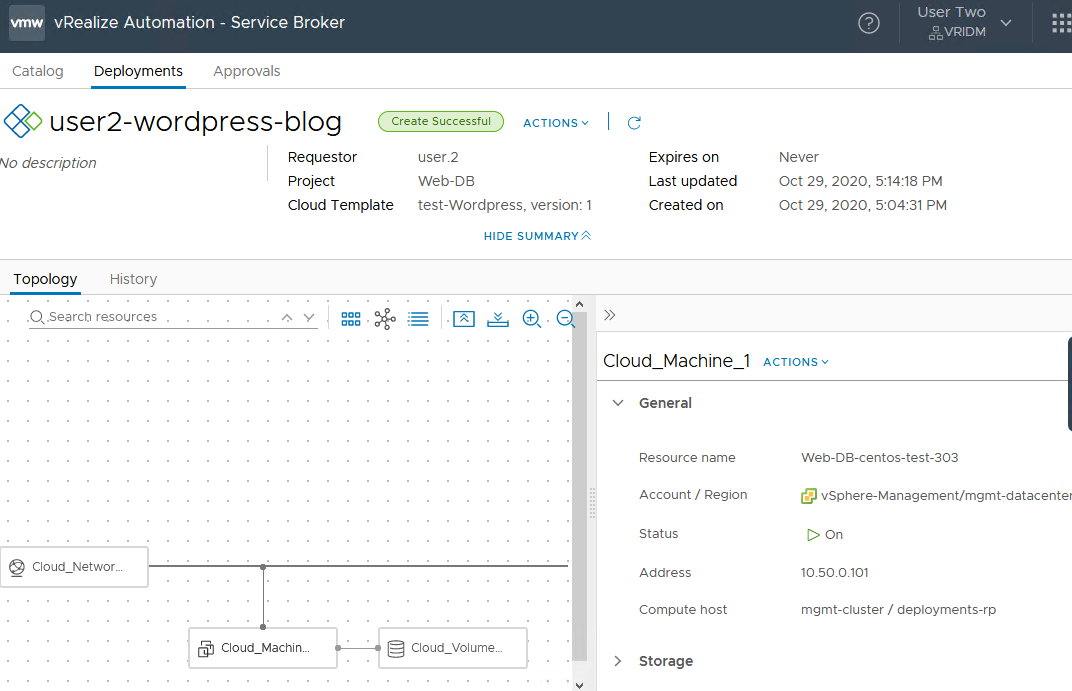
\includegraphics[width=0.8\textwidth]{imaxes/pruebaconcepto/vrealize/user-2-deploy-fin.png}
            \caption{Panel de control del despliegue iniciado por \textit{User Two} una vez finalizado.}
            \label{fig:control-panel-user2}
        \end{figure}
        \FloatBarrier
        \begin{figure}[h]
            \centering
            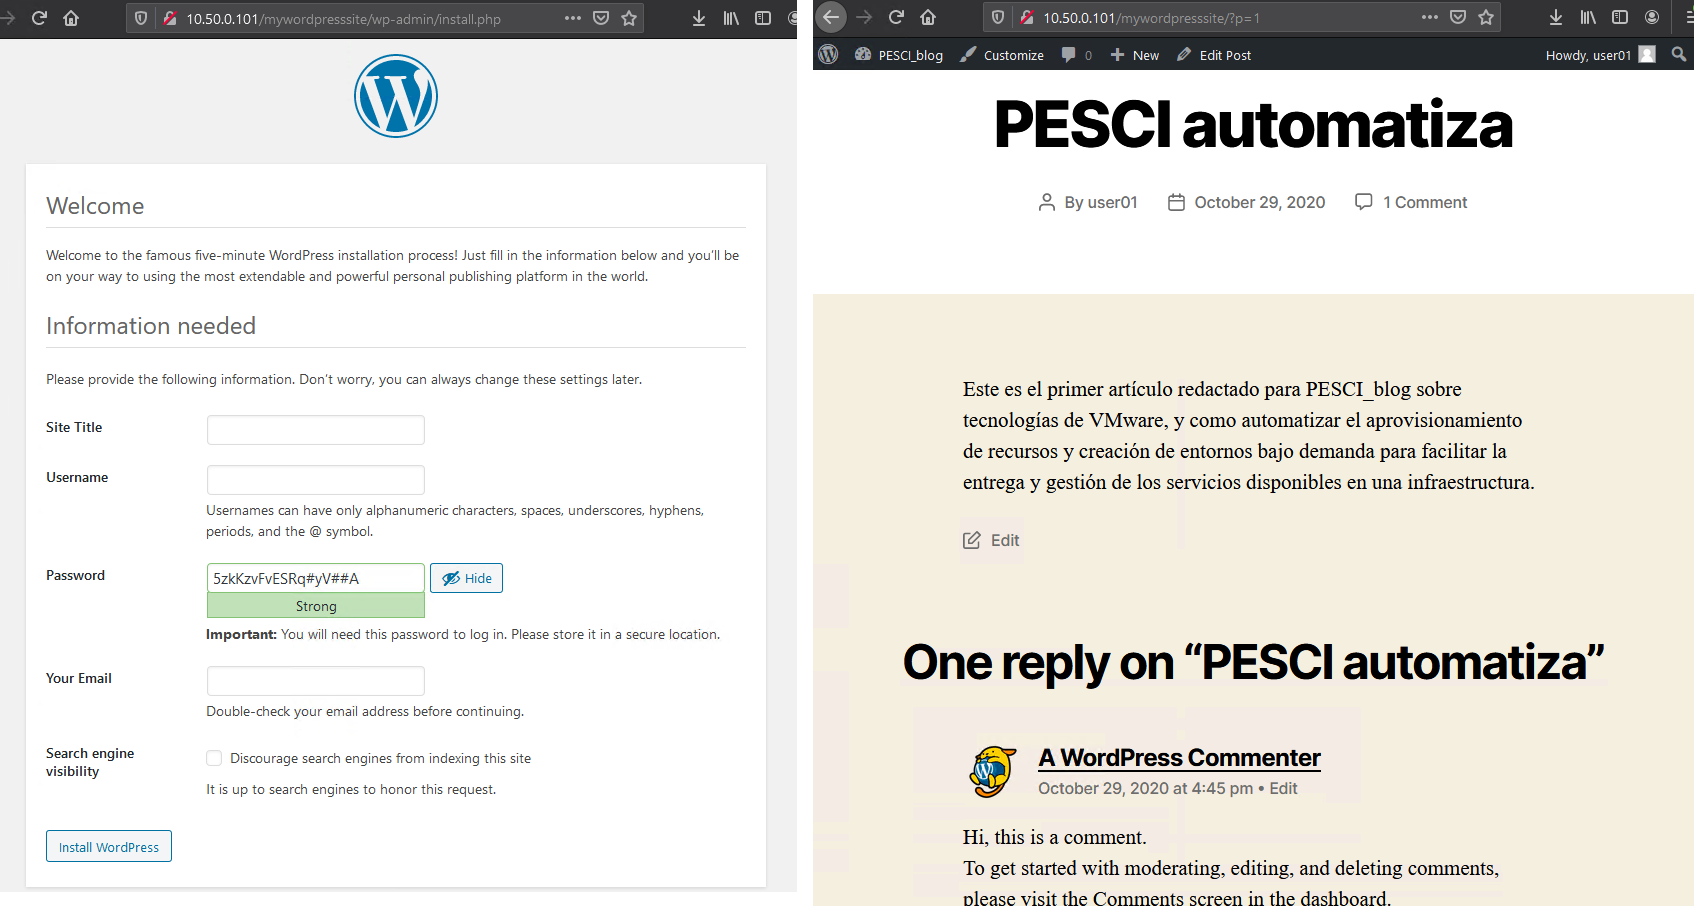
\includegraphics[width=0.8\textwidth]{imaxes/pruebaconcepto/vrealize/wordpress-installation.png}
            \caption{Página de instalación de Worpress cuando \textit{User Three} accede por primera vez (izquierda). Primer artículo escrito por \textit{User Two} en su nuevo sitio web.}
            \label{fig:wordpress-user-2}
        \end{figure}
        \FloatBarrier
        % Despliegue iniciado por \textit{User Two} finalizado junto con la información sobre la VM generada (derecha)
        % Desde el componente Cloud Assembly de vRA, el administrador crea los dos proyectos y asigna respectivamente el rol Administrador de Poryecto a los usuarios \textit{Manager One} y \textit{Manager Two}, mientras que el resto de usuarios reciben el rol Miembro de Proyecto. Con esta asignación cada usuario solo podrá acceder a los proyectos donde se le haya asignado un rol, lo cual podrán hacer a través del componente Service Broker de vRA.
        % El administrador de cada proyecto se encargará del diseño de blueprints, de habilitar las blueprints en el catálogo del proyecto y de controlar los usuarios que son miembros del proyecto. Los miembros del proyecto podrán realizar despliegues a partir de las blueprints habilitadas por el administrador del proyecto.
        A medida que se despliegan los diseños las VMs creadas comienzan a consumir recursos. El administrador del SDDC y los usuarios pueden monitorizar el consumo desde el panel de control de cada despliegue, donde pueden acceder a estadísticas diarias, semanales y mensuales sobre el uso de CPU, memoria RAM, almacenamiento y red.
        \begin{figure}[h]
            \centering
            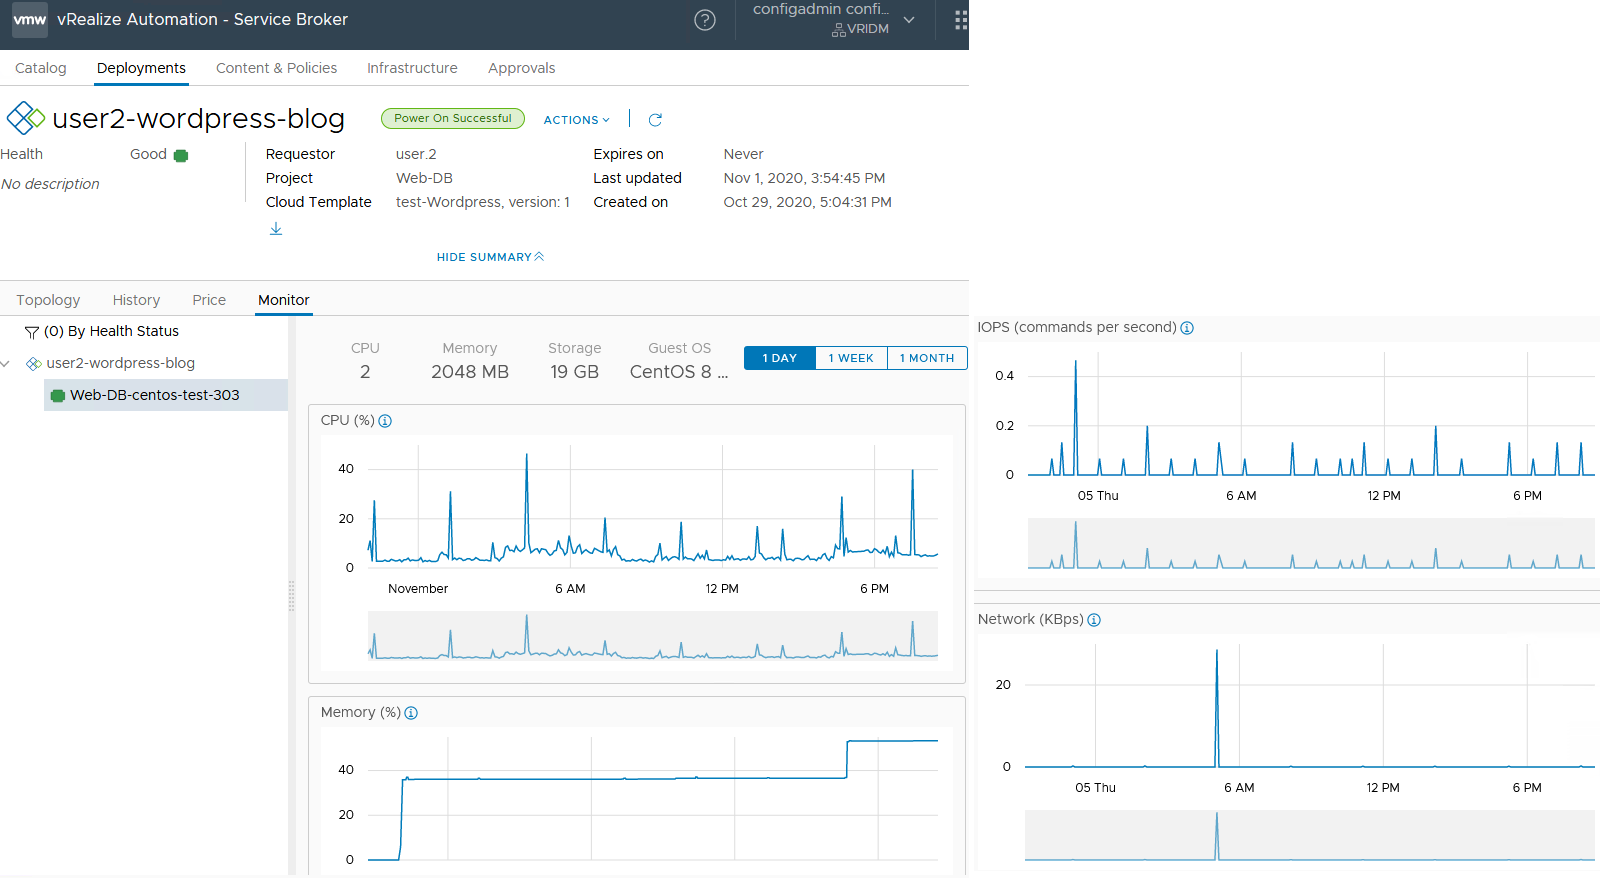
\includegraphics[width=0.8\textwidth]{imaxes/pruebaconcepto/vrealize/statistics-service-broker.png}
            \caption{Panel de control del despliegue User2-Wordpress-Blog con la vista de monitorización de la VM Web-DB-CentOS-test-303.}
            \label{fig:statistics-user-2}
        \end{figure}
        \FloatBarrier
        Una vez el despliegue ha estado cierto tiempo activo, alrededor de un día, en el panel de control del despliegue se empiezan a mostrar estadísticas sobre el coste que tiene el consumo de recursos realizado. El cálculo es realizado por el componente vROps en base a la tarjeta de cobro establecida previamente, la cantidad de recursos utilizada y al tiempo de actividad del despliegue. Posteriormente, vROps comunica esta información a vRA que muestra al usuario todos los detalles.
        \begin{figure}[h]
            \centering
            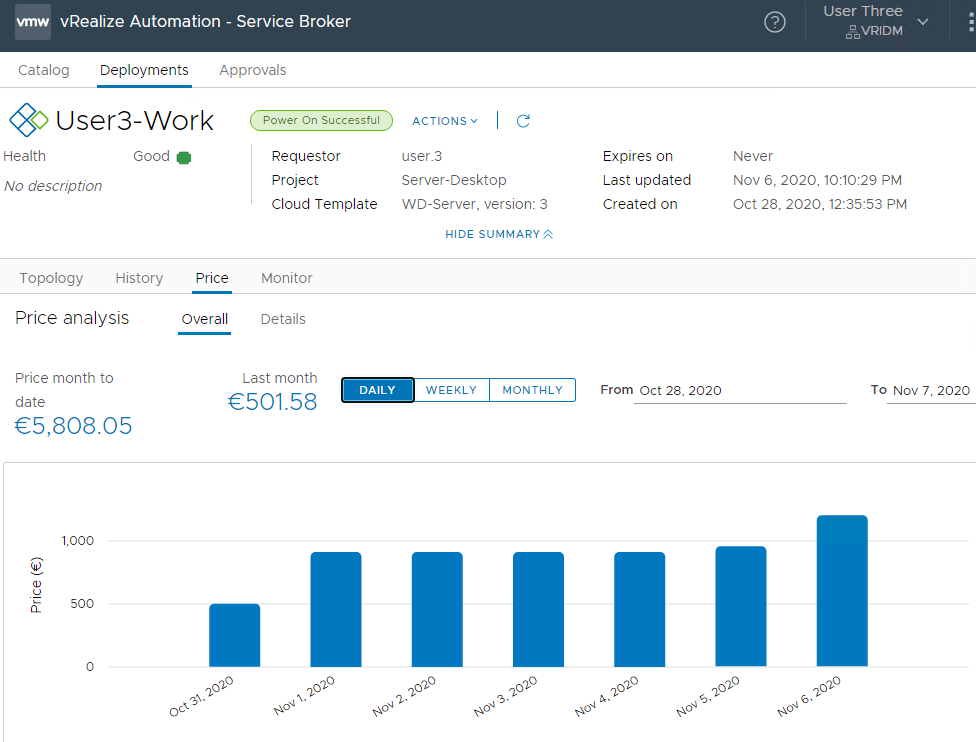
\includegraphics[width=0.7\textwidth]{imaxes/pruebaconcepto/vrealize/price-user3-work.png}
            \caption{Estadística del coste diario de los recursos consumidos en el despliegue User3-Work por parte del usuario \textit{User Three}.}
            \label{fig:user3-daily-price}
        \end{figure}
        \FloatBarrier
        \begin{figure}[h]
            \centering
            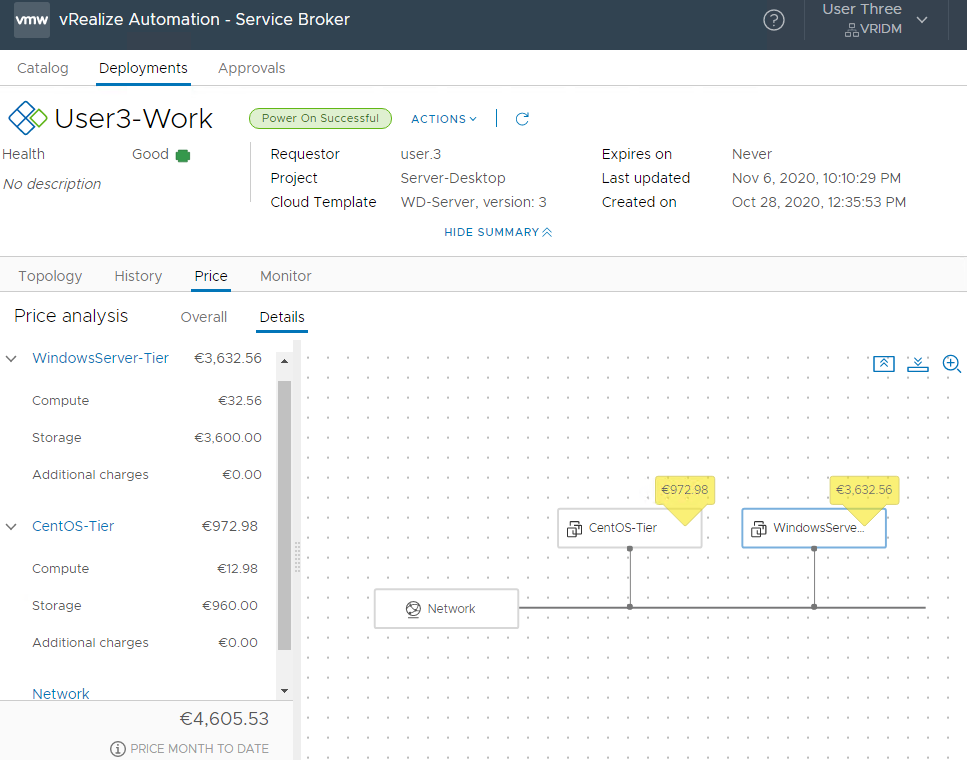
\includegraphics[width=0.7\textwidth]{imaxes/pruebaconcepto/vrealize/user3-price-details.png}
            \caption{Estadística del coste detallado de los recursos consumidos en el despliegue User3-Work por parte del usuario \textit{User Three}.}
            \label{fig:user3-detail-price}
        \end{figure}
        \FloatBarrier
        Como se muestra en la figura \ref{fig:user3-daily-price}, el usuario \textit{User Three} accede a las estadísticas de coste de su despliegue a través de la pestaña "Price" en el panel de control. Aquí obtiene el coste diario, semanal, mensual y total de los recursos que ha consumido. En la figura \ref{fig:user3-detail-price} se muestra el desglose del coste total para que el usuario pueda conocer el coste de cada elemento desplegado.
        \begin{figure}[h]
            \centering
            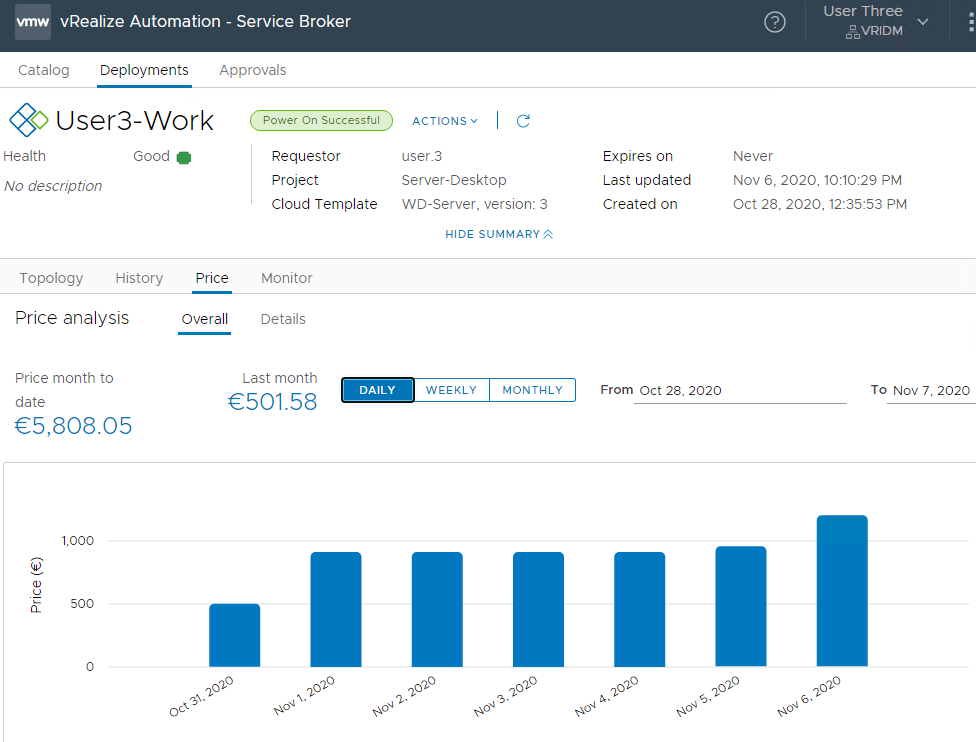
\includegraphics[width=0.7\textwidth]{imaxes/pruebaconcepto/vrealize/price-user3-work.png}
            \caption{Estadística del coste diario de los recursos consumidos en el despliegue User2-Wordpress-Blog por parte del usuario \textit{User Two}.}
            \label{fig:user2-daily-price}
        \end{figure}
        \FloatBarrier
        \begin{figure}[h]
            \centering
            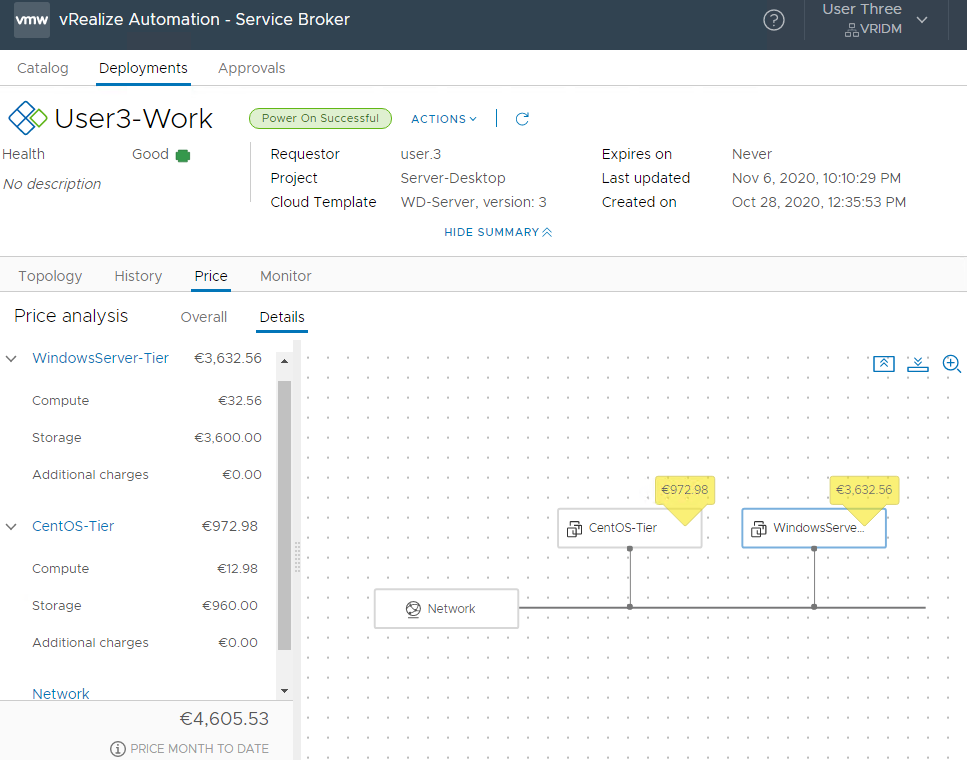
\includegraphics[width=0.7\textwidth]{imaxes/pruebaconcepto/vrealize/user3-price-details.png}
            \caption{Estadística del coste detallado de los recursos consumidos en el despliegue User2-Wordpress-Blog por parte del usuario \textit{User Two}.}
            \label{fig:user2-detail-price}
        \end{figure}
        \FloatBarrier
        El administrador del SDDC aparte de tener acceso a todos los despliegues realizados en el vRA, desde vROps también puede obtener las estadísticas sobre el coste de los recursos consumidos pero de forma algo más detallada. Desde este componente el administrador del SDDC puede ver el coste total y detallado de cada proyecto y de los despliegues realizados en cada uno (figuras \ref{fig:vrops-cost-projects}, \ref{fig:vrops-cost-user3} y \ref{fig:vrops-cost-user2}). Además, también tiene acceso a gráficos donde se muestra el coste realizado en cada proyecto y despliegue a lo largo del tiempo, y una predicción del coste en los siguientes cinco días según el estado de cada despliegue (figuras \ref{fig:vrops-graf-user3} y \ref{fig:vrops-graf-user2}).
        \begin{figure}[h]
            \centering
            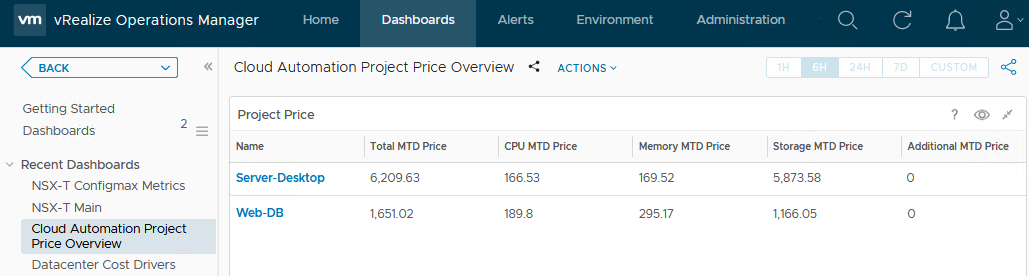
\includegraphics[width=0.7\textwidth]{imaxes/pruebaconcepto/vrealize/vrops-projects-price.png}
            \caption{Información sobre el coste de los proyectos Server-Desktop y Web-DB ofrecida por vROps.}
            \label{fig:vrops-cost-projects}
        \end{figure}
        \FloatBarrier
        \begin{figure}[h]
            \centering
            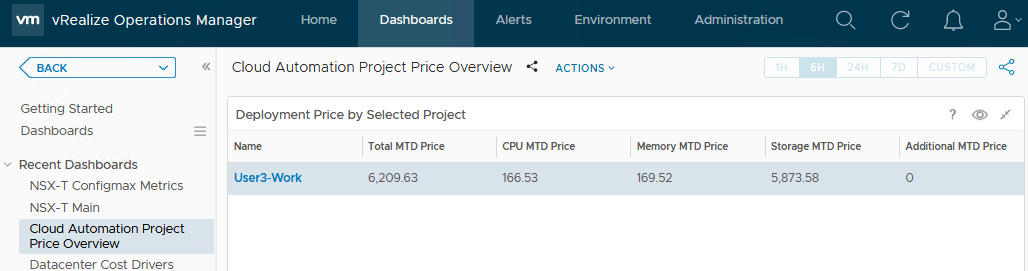
\includegraphics[width=0.7\textwidth]{imaxes/pruebaconcepto/vrealize/vrops-user3-price.png}
            \caption{Información sobre el coste del despliegue User3-Work del usuario \textit{User Three} ofrecida por vROps.}
            \label{fig:vrops-cost-user3}
        \end{figure}
        \FloatBarrier
        \begin{figure}[h]
            \centering
            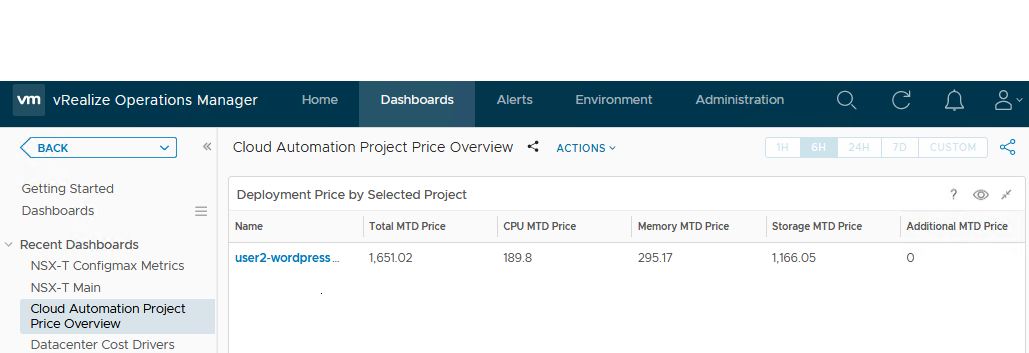
\includegraphics[width=0.7\textwidth]{imaxes/pruebaconcepto/vrealize/vrops-user2-price.png}
            \caption{Información sobre el coste del despliegue User2-Wordpress-Blog del usuario \textit{User Two} ofrecida por vROps.}
            \label{fig:vrops-cost-user2}
        \end{figure}
        \FloatBarrier
        \begin{figure}[h]
            \centering
            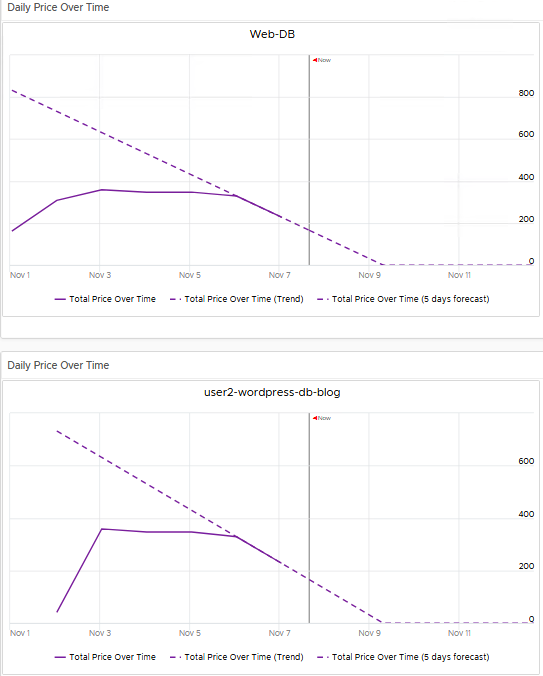
\includegraphics[width=0.7\textwidth]{imaxes/pruebaconcepto/vrealize/vrops-graf-user2.png}
            \caption{Gráfico de coste del proyecto Web-DB y del despliegue User2-Wordpress-Blog del usuario \textit{User Two} ofrecido por vROps.}
            \label{fig:vrops-graf-user2}
        \end{figure}
        \FloatBarrier
        \begin{figure}[h]
            \centering
            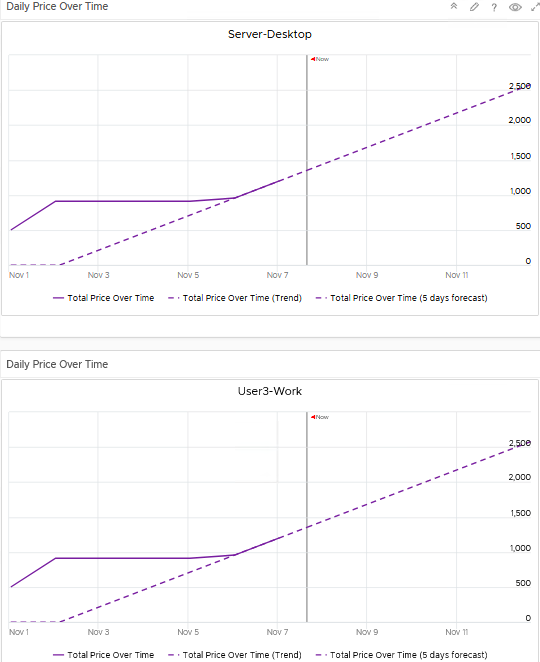
\includegraphics[width=0.7\textwidth]{imaxes/pruebaconcepto/vrealize/vrops-graf-user3.png}
            \caption{Gráfico de coste del proyecto Server-Desktop y del despliegue User3-Work del usuario \textit{User Three} ofrecido por vROps.}
            \label{fig:vrops-graf-user3}
        \end{figure}
        \FloatBarrier
        De esta forma el administrador del SDDC puede asignar a cada proyecto o usuario una cuenta con una cantidad de dinero ficticio de la cual se va extrayendo de forma mensual o semanal el coste del consumo realizado. Cuando la cuenta esté vacía o no tenga suficiente saldo para consumir más recursos el administrador del SDDC puede bloquear nuevos despliegues para un proyecto o usuario de forma temporal  hasta que su cuenta vuelva a tener saldo. Con este método se persigue que el servicio tenga recursos suficientes para todos los usuarios y para ejecutar los flujos de trabajo de forma correcta, y evitar que existan usuarios con despliegues activos pero que no están siendo realmente usados.

        Además, desde vROps el administrador también tiene visibilidad sobre los eventos que suceden en la infraestructura y estadísticas sobre los recursos, como se muestra en las dos siguientes figuras.
        \begin{figure}[h]
            \centering
            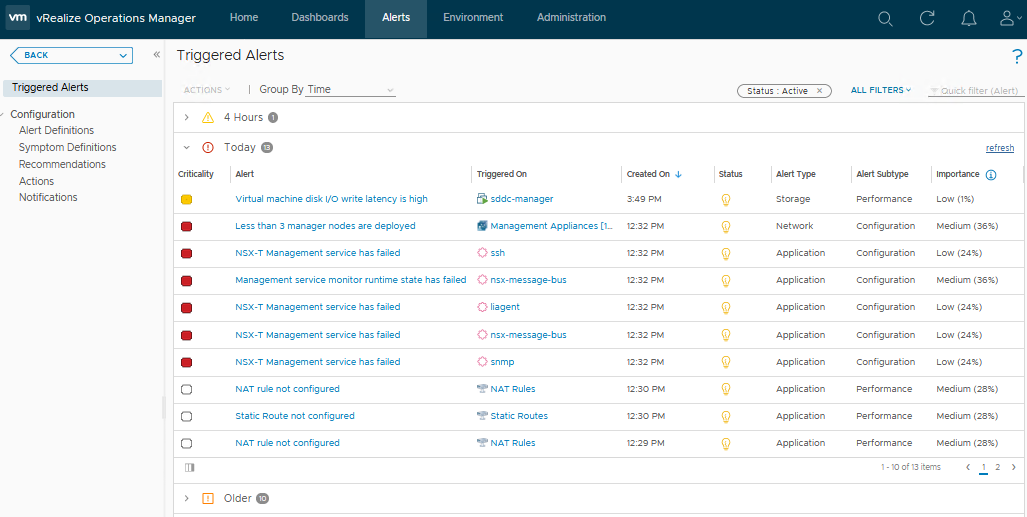
\includegraphics[width=0.6\textwidth]{imaxes/pruebaconcepto/vrealize/vrops-alerts.png}
            \caption{Alertas ocurridas en la infraestructura con información sobre su gravedad.}
            \label{fig:vrops-alerts}
        \end{figure}
        \FloatBarrier
        \begin{figure}[h]
            \centering
            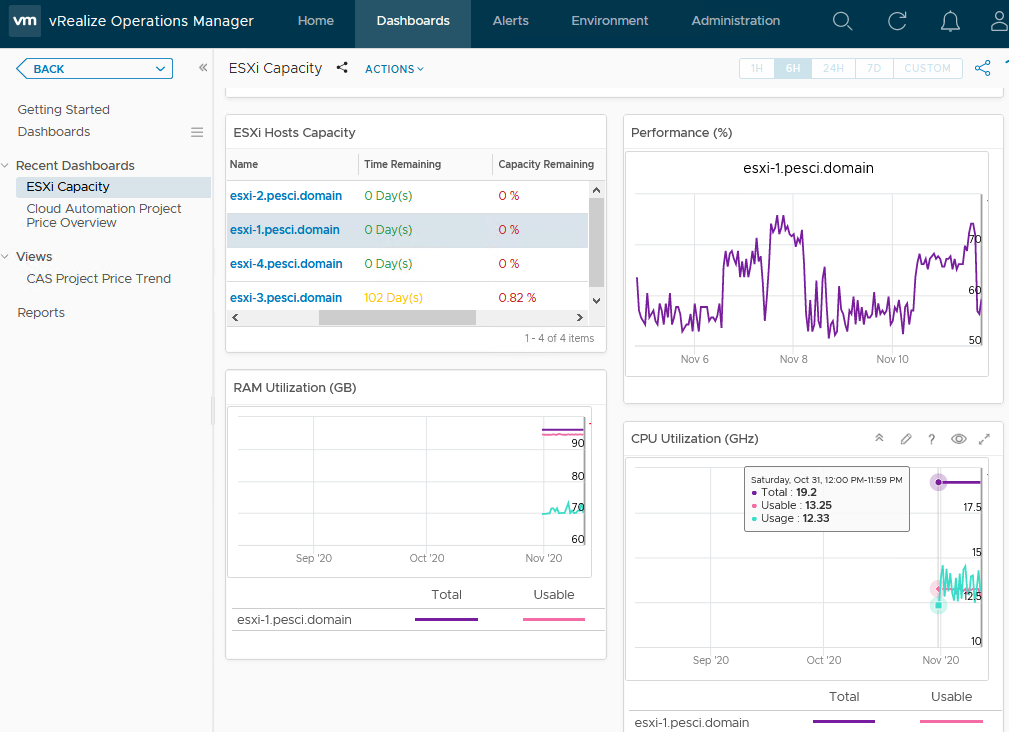
\includegraphics[width=0.6\textwidth]{imaxes/pruebaconcepto/vrealize/vrops-statistics.png}
            \caption{Estadísticas sobre la cantidad de recursos utilizados en cada host del entorno a lo largo del tiempo.}
            \label{fig:vrops-statistics}
        \end{figure}
        \FloatBarrier

        Habiendo cumplido todos los objetivos de este proyecto se concluye la formación de un servicio Cloud para la infraestructura del CITIC, usable por sus usuarios y capaz de optimizar el uso de los recursos.
        % Las estadísticas en cuanto a la valoración de los recursos en base a la tarjeta de cobro establecida también es accedida desde el panel de control del despliegue bajo la pestaña "Price". En ella los usuarios pueden ver la valoración total diaria, semanal y mensual de los recursos consumidos en el despliegue, y también de forma detallada donde se desglosa la valoración total en la valoración del cómputo, almacenamiento y otros cargos adicionales que se puedan aplicar. Además, el administrador del SDDC también tiene acceso a estadísticas sobre la valoración total sobre el consumo de recursos de un proyecto.
    \end{subsubsection}
    
    % Para ordenar el aprovisionamiento de los recursos, antes de realizar cualquier implementación, es necesario configurar la infraestructura que se va a poner a disposición de los usuarios. 
    %     En VMware vCenter Server, dentro del cluster vSphere se define un \textit{resource pool} y una carpeta que se utilizarán para colocar las VMs que se desplieguen desde vRA. 
    %     La red que utilizarán las VMs generadas estará controlada por VMware NSX-T para aprovechar las ventajas de sus redes definidas por software y así automatizar su configuración y hacer uso de los servicios que ofrece. Para ello se añade un Segment al router virtual de Tier-1 que se muestra en la figura \ref{fig:two-tier-topology}, VMware NSX-T informa de la nueva ruta al router físico mediante BGP proporcionando así acceso a redes externas.
    %     \begin{figure}[h]
    %         \centering
    %         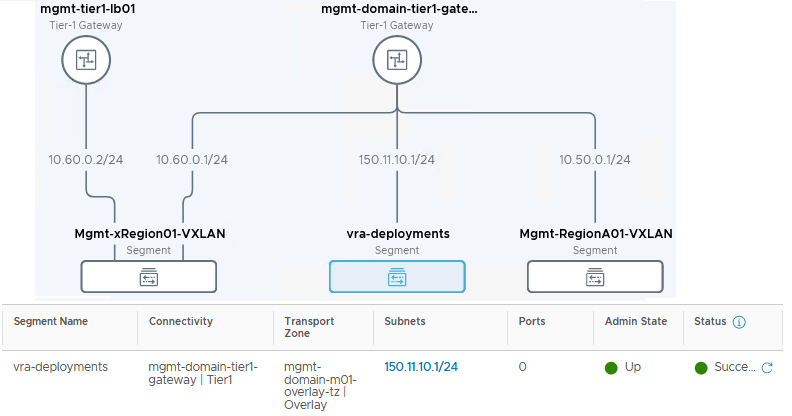
\includegraphics[width=0.4\textwidth]{imaxes/pruebaconcepto/vrealize/topology-for-vRA-NSXT.png}
    %         \caption{Nuevo Segment \textit{vra-deployments} en el router virtual Tier-1.}
    %         \label{fig:topology-nsx-t-vra}
    %     \end{figure}
    %     \FloatBarrier
    %     Las VMs que los usuarios generan están basadas en plantillas que son creadas previamente por el administrador. Antes de generar la plantilla el administrador debe crear una VM en VMware vCenter Server y proveerla con una configuración mínima para que el usuario pueda aplicar su propia configuración durante el despliegue, para este entorno se crea una VM con el sistema operativo Ubuntu Server 20.04.1. Una vez se termina el proceso de instalación y actualización del sistema operativo, se configura el servicio \textbf{cloud-init}\footnote{Se puede encontrar más información sobre cloud-init en el enlace: \url{https://cloudinit.readthedocs.io/en/latest/}} el cual permite inicializar la VM con la configuración indicada en la blueprint, como se verá más adelante. También se pueden preinstalar servicios como bases de datos para que el usuario solo tenga que configurarlo. Cuando la configuración de la VM está lista, se limpia limpian el hostname, archivos de logs, claves SSH y caché del servicio cloud-init ejecutando el siguiente script, para que en cada implementación se genere una VM distinta a partir de la misma plantilla. Finalmente, la VM se convierte a una plantilla que se almacena en VMware vCenter Server.
    %     \begin{figure}[h]
    %         \centering
    %         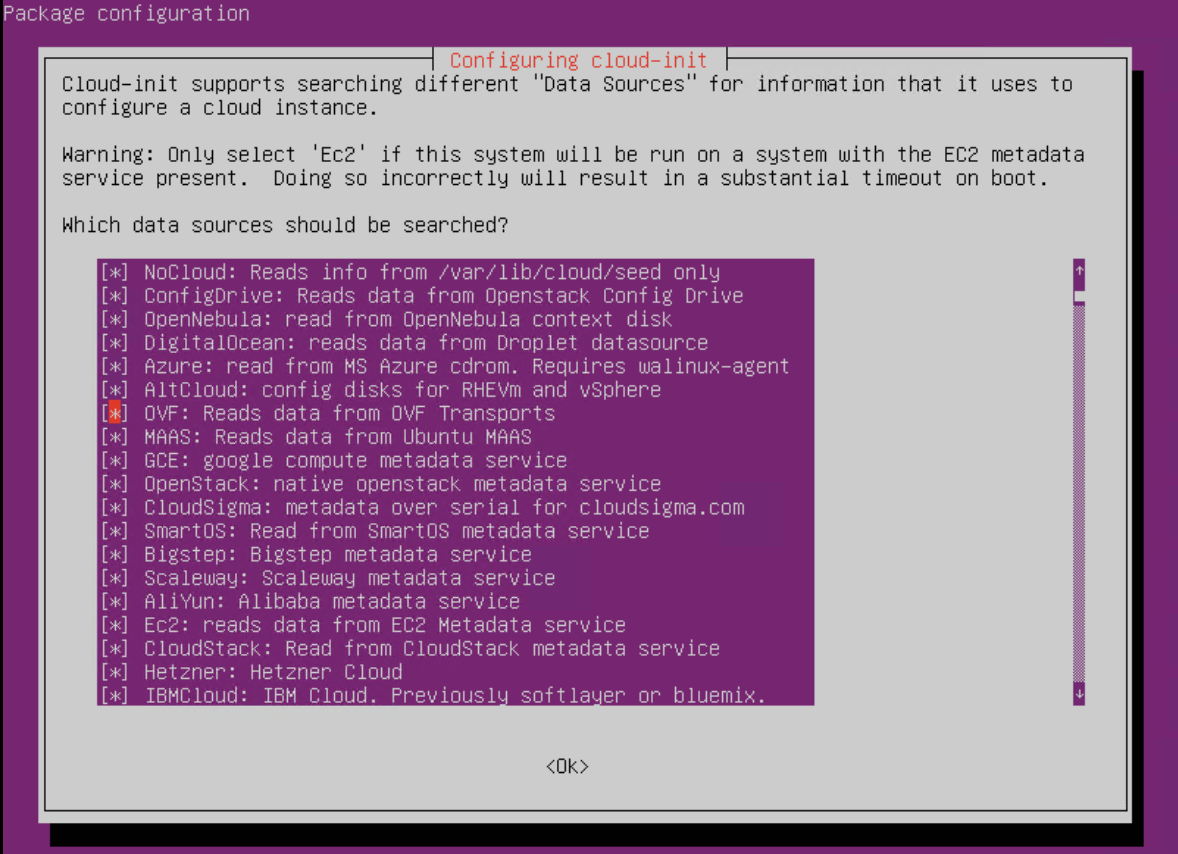
\includegraphics[width=0.4\textwidth]{imaxes/pruebaconcepto/vrealize/install-cloud-init.png}
    %         \caption{Configuración del servicio cloud-init en Ubuntu Server 20.}
    %         \label{fig:cloud-init-config}
    %     \end{figure}
    %     \FloatBarrier
    %     \begin{figure}[h]
    %         \centering
    %         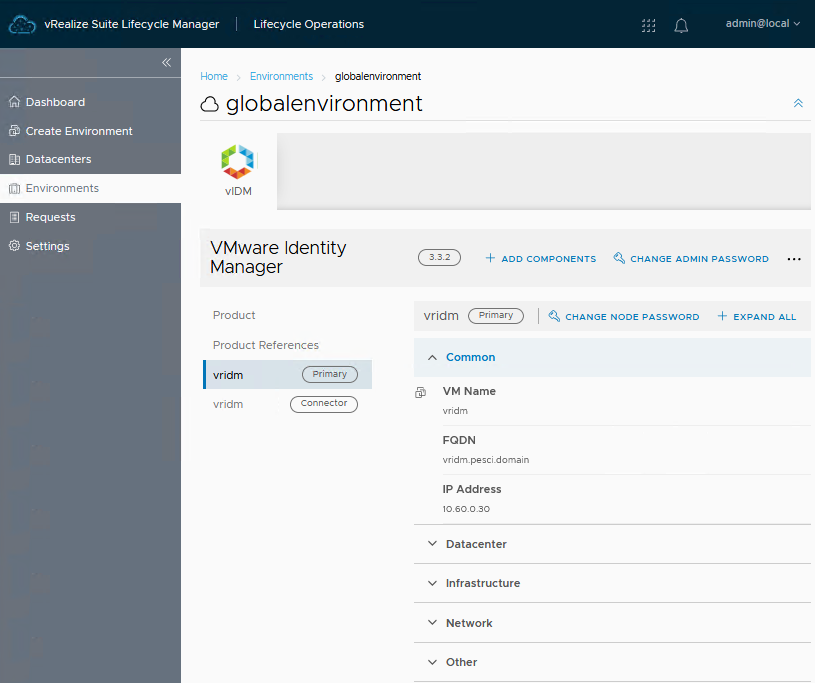
\includegraphics[width=0.4\textwidth]{imaxes/pruebaconcepto/vrealize/config-istance-vridm.png}
    %         \caption{Creación de una plantilla a partir de la VM de Ubuntu Server 20.}
    %         \label{fig:template-ubuntu}
    %     \end{figure}
    %     \FloatBarrier

    %     Una vez se tienen los recursos que serán usados por los usuarios es necesario añadirlos a vRA. Para poder esos recursos, durante su configuración vRA se asigna un tag a cada uno con la forma \textit{key:value}. En una blueprint estos tags permitirán indicar a que recurso se está refiriendo. 
    %     Lo primero es configurar una Cloud Zone que proporcionará acceso a todos los recursos situados en el cluster vSphere. El tag utilizado para esta será \textit{cloud:private}. Posteriormente se definen los tamaños de VMs que se habilitan, también llamado Flavour Mapping. Se configuran cuatro tamaños, X-small (1 CPU y 512 MB de RAM), Small (2 CPU y 8 GB de RAM), Medium (8 CPU y 4 GB de RAM) y Large (8 CPU y 16 GB de RAM). Las redes disponibles se añaden mediante la creación de perfiles donde se definen los tags con los que se identifica la red, su gateway, su servidor DNS, el rango de IPs para asignar una IP a cada VM conectada a esa red. 
\end{subsection}